\documentclass[twoside]{book}

% Packages required by doxygen
\usepackage{fixltx2e}
\usepackage{calc}
\usepackage{doxygen}
\usepackage[export]{adjustbox} % also loads graphicx
\usepackage{graphicx}
\usepackage[utf8]{inputenc}
\usepackage{makeidx}
\usepackage{multicol}
\usepackage{multirow}
\PassOptionsToPackage{warn}{textcomp}
\usepackage{textcomp}
\usepackage[nointegrals]{wasysym}
\usepackage[table]{xcolor}

% Font selection
\usepackage[T1]{fontenc}
\usepackage[scaled=.90]{helvet}
\usepackage{courier}
\usepackage{amssymb}
\usepackage{sectsty}
\renewcommand{\familydefault}{\sfdefault}
\allsectionsfont{%
  \fontseries{bc}\selectfont%
  \color{darkgray}%
}
\renewcommand{\DoxyLabelFont}{%
  \fontseries{bc}\selectfont%
  \color{darkgray}%
}
\newcommand{\+}{\discretionary{\mbox{\scriptsize$\hookleftarrow$}}{}{}}

% Page & text layout
\usepackage{geometry}
\geometry{%
  a4paper,%
  top=2.5cm,%
  bottom=2.5cm,%
  left=2.5cm,%
  right=2.5cm%
}
\tolerance=750
\hfuzz=15pt
\hbadness=750
\setlength{\emergencystretch}{15pt}
\setlength{\parindent}{0cm}
\setlength{\parskip}{3ex plus 2ex minus 2ex}
\makeatletter
\renewcommand{\paragraph}{%
  \@startsection{paragraph}{4}{0ex}{-1.0ex}{1.0ex}{%
    \normalfont\normalsize\bfseries\SS@parafont%
  }%
}
\renewcommand{\subparagraph}{%
  \@startsection{subparagraph}{5}{0ex}{-1.0ex}{1.0ex}{%
    \normalfont\normalsize\bfseries\SS@subparafont%
  }%
}
\makeatother

% Headers & footers
\usepackage{fancyhdr}
\pagestyle{fancyplain}
\fancyhead[LE]{\fancyplain{}{\bfseries\thepage}}
\fancyhead[CE]{\fancyplain{}{}}
\fancyhead[RE]{\fancyplain{}{\bfseries\leftmark}}
\fancyhead[LO]{\fancyplain{}{\bfseries\rightmark}}
\fancyhead[CO]{\fancyplain{}{}}
\fancyhead[RO]{\fancyplain{}{\bfseries\thepage}}
\fancyfoot[LE]{\fancyplain{}{}}
\fancyfoot[CE]{\fancyplain{}{}}
\fancyfoot[RE]{\fancyplain{}{\bfseries\scriptsize Generated by Doxygen }}
\fancyfoot[LO]{\fancyplain{}{\bfseries\scriptsize Generated by Doxygen }}
\fancyfoot[CO]{\fancyplain{}{}}
\fancyfoot[RO]{\fancyplain{}{}}
\renewcommand{\footrulewidth}{0.4pt}
\renewcommand{\chaptermark}[1]{%
  \markboth{#1}{}%
}
\renewcommand{\sectionmark}[1]{%
  \markright{\thesection\ #1}%
}

% Indices & bibliography
\usepackage{natbib}
\usepackage[titles]{tocloft}
\setcounter{tocdepth}{3}
\setcounter{secnumdepth}{5}
\makeindex

% Hyperlinks (required, but should be loaded last)
\usepackage{ifpdf}
\ifpdf
  \usepackage[pdftex,pagebackref=true]{hyperref}
\else
  \usepackage[ps2pdf,pagebackref=true]{hyperref}
\fi
\hypersetup{%
  colorlinks=true,%
  linkcolor=blue,%
  citecolor=blue,%
  unicode%
}

% Custom commands
\newcommand{\clearemptydoublepage}{%
  \newpage{\pagestyle{empty}\cleardoublepage}%
}

\usepackage{caption}
\captionsetup{labelsep=space,justification=centering,font={bf},singlelinecheck=off,skip=4pt,position=top}

%===== C O N T E N T S =====

\begin{document}

% Titlepage & ToC
\hypersetup{pageanchor=false,
             bookmarksnumbered=true,
             pdfencoding=unicode
            }
\pagenumbering{alph}
\begin{titlepage}
\vspace*{7cm}
\begin{center}%
{\Large M\+\_\+time }\\
\vspace*{1cm}
{\large Generated by Doxygen 1.8.14}\\
\end{center}
\end{titlepage}
\clearemptydoublepage
\pagenumbering{roman}
\tableofcontents
\clearemptydoublepage
\pagenumbering{arabic}
\hypersetup{pageanchor=true}

%--- Begin generated contents ---
\chapter{M\+\_\+\+C\+LI Fortran Library}
\label{index}\hypertarget{index}{}    

    \hypertarget{index_Introduction}{}\section{Introduction}\label{index_Introduction}
command line parsing using N\+A\+M\+E\+L\+I\+ST groups

      
\chapter{Modules Index}
\section{Modules List}
Here is a list of all modules with brief descriptions\+:\begin{DoxyCompactList}
\item\contentsline{section}{\mbox{\hyperlink{namespacem__cli}{m\+\_\+cli}} }{\pageref{namespacem__cli}}{}
\end{DoxyCompactList}

\chapter{Data Type Index}
\section{Data Types List}
Here are the data types with brief descriptions\+:\begin{DoxyCompactList}
\item\contentsline{section}{\mbox{\hyperlink{structm__cli_1_1dictionary}{m\+\_\+cli\+::dictionary}} }{\pageref{structm__cli_1_1dictionary}}{}
\item\contentsline{section}{\mbox{\hyperlink{interfacem__cli_1_1insert}{m\+\_\+cli\+::insert}} }{\pageref{interfacem__cli_1_1insert}}{}
\item\contentsline{section}{\mbox{\hyperlink{interfacem__cli_1_1locate}{m\+\_\+cli\+::locate}} }{\pageref{interfacem__cli_1_1locate}}{}
\item\contentsline{section}{\mbox{\hyperlink{structm__cli_1_1option}{m\+\_\+cli\+::option}} }{\pageref{structm__cli_1_1option}}{}
\item\contentsline{section}{\mbox{\hyperlink{interfacem__cli_1_1remove}{m\+\_\+cli\+::remove}} }{\pageref{interfacem__cli_1_1remove}}{}
\item\contentsline{section}{\mbox{\hyperlink{interfacem__cli_1_1replace}{m\+\_\+cli\+::replace}} }{\pageref{interfacem__cli_1_1replace}}{}
\end{DoxyCompactList}

\chapter{File Index}
\section{File List}
Here is a list of all files with brief descriptions\+:\begin{DoxyCompactList}
\item\contentsline{section}{/home/urbanjs/venus/\+V600/github/\+M\+\_\+\+C\+L\+I/src/\mbox{\hyperlink{M__CLI_8f90}{M\+\_\+\+C\+L\+I.\+f90}} }{\pageref{M__CLI_8f90}}{}
\end{DoxyCompactList}

\chapter{Module Documentation}
\hypertarget{namespacem__cli}{}\section{m\+\_\+cli Module Reference}
\label{namespacem__cli}\index{m\+\_\+cli@{m\+\_\+cli}}
\subsection*{Data Types}
\begin{DoxyCompactItemize}
\item 
type \mbox{\hyperlink{structm__cli_1_1dictionary}{dictionary}}
\item 
interface \mbox{\hyperlink{interfacem__cli_1_1insert}{insert}}
\item 
interface \mbox{\hyperlink{interfacem__cli_1_1locate}{locate}}
\item 
type \mbox{\hyperlink{structm__cli_1_1option}{option}}
\item 
interface \mbox{\hyperlink{interfacem__cli_1_1remove}{remove}}
\item 
interface \mbox{\hyperlink{interfacem__cli_1_1replace}{replace}}
\end{DoxyCompactItemize}
\subsection*{Functions/\+Subroutines}
\begin{DoxyCompactItemize}
\item 
subroutine, public \mbox{\hyperlink{namespacem__cli_a62056f0c153eb63cb0b11a21edb028cd}{check\+\_\+commandline}} (ios, message, help\+\_\+text, version\+\_\+text)
\item 
character(len=\+:) function, allocatable, public \mbox{\hyperlink{namespacem__cli_a4f639b0c4bf16930fc1c5858ed4196a3}{commandline}} (definition, name, noquote)
\item 
subroutine, private \mbox{\hyperlink{namespacem__cli_a8c62537a2d224364c9cb30005be819e9}{prototype\+\_\+to\+\_\+dictionary}} (string)
\item 
subroutine, private \mbox{\hyperlink{namespacem__cli_a9b7676d796e5cb878ecd9294b8a689cb}{update}} (key, val)
\item 
subroutine, private \mbox{\hyperlink{namespacem__cli_a3c1b30406fc692841826be979726bb1b}{wipe\+\_\+dictionary}} ()
\item 
character(len=\+:) function, allocatable, private \mbox{\hyperlink{namespacem__cli_a45783c194a1484042f63c58b180ca8df}{get}} (key)
\item 
subroutine, private \mbox{\hyperlink{namespacem__cli_ac77d70573b34ade2079cc4004a6acba5}{prototype\+\_\+and\+\_\+cmd\+\_\+args\+\_\+to\+\_\+nlist}} (prototype, nml)
\item 
subroutine \mbox{\hyperlink{namespacem__cli_a89a63254465b02048f09541e51974764}{cmd\+\_\+args\+\_\+to\+\_\+dictionary}} (check)
\item 
subroutine \mbox{\hyperlink{namespacem__cli_a7e5041efcad56387232475a3ae728634}{dictionary\+\_\+to\+\_\+namelist}} (nml)
\item 
subroutine, public \mbox{\hyperlink{namespacem__cli_a5b6abaf1d5aec5e918be0759df29c849}{print\+\_\+dictionary}} (header, stop)
\item 
integer function, private \mbox{\hyperlink{namespacem__cli_aaf5504d3b48696a9d22fa5773c5a7d15}{longest\+\_\+command\+\_\+argument}} ()
\item 
subroutine, private \mbox{\hyperlink{namespacem__cli_ade3d1e36f0fc6a47b5469dcd8ade5312}{locate\+\_\+c}} (list, value, place, ier, errmsg)
\item 
subroutine, private \mbox{\hyperlink{namespacem__cli_a4187c24a2abf5cc630232965637493e8}{locate\+\_\+d}} (list, value, place, ier, errmsg)
\item 
subroutine, private \mbox{\hyperlink{namespacem__cli_ac44389e115b536069f324bffea7d2469}{locate\+\_\+r}} (list, value, place, ier, errmsg)
\item 
subroutine, private \mbox{\hyperlink{namespacem__cli_a36665ab0ea5080c14c8c9e52ed07d397}{locate\+\_\+i}} (list, value, place, ier, errmsg)
\item 
subroutine, private \mbox{\hyperlink{namespacem__cli_a05f549b10f50798d68003b8fd2a2d86a}{remove\+\_\+c}} (list, place)
\item 
subroutine, private \mbox{\hyperlink{namespacem__cli_abf22cbc2af66482f33b7bb1a210d9d99}{remove\+\_\+d}} (list, place)
\item 
subroutine, private \mbox{\hyperlink{namespacem__cli_a4f47701695b95c88fa4927c04996ce0f}{remove\+\_\+r}} (list, place)
\item 
subroutine, private \mbox{\hyperlink{namespacem__cli_a9c86f0f52ce71f14e774fd21f0686cf6}{remove\+\_\+l}} (list, place)
\item 
subroutine, private \mbox{\hyperlink{namespacem__cli_afa08d3d87184a6dd68a124231e536c93}{remove\+\_\+i}} (list, place)
\item 
subroutine, private \mbox{\hyperlink{namespacem__cli_a785aa0016768b6dc2e27c29d5342c329}{replace\+\_\+c}} (list, value, place)
\item 
subroutine, private \mbox{\hyperlink{namespacem__cli_aa9b7d672cc9fb0bc79fd09a2870614f5}{replace\+\_\+d}} (list, value, place)
\item 
subroutine, private \mbox{\hyperlink{namespacem__cli_ab3b33abc8a6da174d3f27c2f2203038c}{replace\+\_\+r}} (list, value, place)
\item 
subroutine, private \mbox{\hyperlink{namespacem__cli_a89ed5c3b944f91d8135173206fbc7e07}{replace\+\_\+l}} (list, value, place)
\item 
subroutine, private \mbox{\hyperlink{namespacem__cli_ac609c48bb1f904235b8cbf8bea61473f}{replace\+\_\+i}} (list, value, place)
\item 
subroutine, private \mbox{\hyperlink{namespacem__cli_a9baf1cf0e20942fbde8c025ead5a30db}{insert\+\_\+c}} (list, value, place)
\item 
subroutine, private \mbox{\hyperlink{namespacem__cli_a4bfb90e14824f94017b1d4fcb39f0701}{insert\+\_\+r}} (list, value, place)
\item 
subroutine, private \mbox{\hyperlink{namespacem__cli_a030e31579a7968aea68d80db1e36ebfd}{insert\+\_\+d}} (list, value, place)
\item 
subroutine, private \mbox{\hyperlink{namespacem__cli_a0c1b22c46470afbb4ee5c67180335578}{insert\+\_\+l}} (list, value, place)
\item 
subroutine, private \mbox{\hyperlink{namespacem__cli_a841685591ef1f1827fc1fe32a7f546f1}{insert\+\_\+i}} (list, value, place)
\item 
subroutine \mbox{\hyperlink{namespacem__cli_aff32e44070983c7fb4eb0a3b1dea7a6d}{dict\+\_\+delete}} (self, key)
\item 
character(len=\+:) function, allocatable \mbox{\hyperlink{namespacem__cli_ac4a889309ffc333af6bf8e11f1fc4869}{dict\+\_\+get}} (self, key)
\item 
subroutine \mbox{\hyperlink{namespacem__cli_a1be098e2b920e8d50ed14be03a3133db}{dict\+\_\+add}} (self, key, value)
\item 
pure elemental logical function \mbox{\hyperlink{namespacem__cli_a4c126288dc18289b2095a0882f10ca77}{isupper}} (ch)
\item 
elemental pure character(len(str)) function \mbox{\hyperlink{namespacem__cli_aef6f54c9cb37251dfd664c0845186a40}{upper}} (str, begin, end)
\item 
elemental pure character(len(str)) function \mbox{\hyperlink{namespacem__cli_a685574282a09c3f57e0c18654a3a642c}{lower}} (str, begin, end)
\item 
character(len=\+:) function, allocatable \mbox{\hyperlink{namespacem__cli_ac82fec2a5441020701fe3c64af3d9948}{quote}} (str, mode)
\item 
character(len=\+:) function, allocatable \mbox{\hyperlink{namespacem__cli_a40e02b1c9fc580ddd410bb24017fab8c}{replace\+\_\+str}} (targetline, old, new, ierr, cmd, range)
\item 
subroutine \mbox{\hyperlink{namespacem__cli_a8d5d1954aac6494e07fb11f12f635c85}{crack\+\_\+cmd}} (cmd, old, new, ierr)
\item 
logical function \mbox{\hyperlink{namespacem__cli_a0015c38f9fa45a58ba6ae89f2ddb54f1}{strtok}} (source\+\_\+string, itoken, token\+\_\+start, token\+\_\+end, delimiters)
\item 
subroutine \mbox{\hyperlink{namespacem__cli_a3b66fe9cee0e084068051636afb2957d}{substitute}} (targetline, old, new, ierr, start, end)
\end{DoxyCompactItemize}
\subsection*{Variables}
\begin{DoxyCompactItemize}
\item 
character(len=\+:), dimension(\+:), allocatable, public \mbox{\hyperlink{namespacem__cli_a7fd43837c254f34109d9f523c66c873a}{unnamed}}
\item 
character(len=\+:), dimension(\+:), allocatable \mbox{\hyperlink{namespacem__cli_a1eb7801692b3d6e25f16885fdf027f42}{keywords}}
\item 
character(len=\+:), dimension(\+:), allocatable \mbox{\hyperlink{namespacem__cli_aaec25aa63c2964c1125b9f14f27bf44a}{values}}
\item 
integer, dimension(\+:), allocatable \mbox{\hyperlink{namespacem__cli_ac6af3775222feedc5aff5874ce63897a}{counts}}
\item 
logical, dimension(\+:), allocatable \mbox{\hyperlink{namespacem__cli_ad08e57d14b3543d476d00e6bfda58fa5}{present\+\_\+in}}
\item 
logical \mbox{\hyperlink{namespacem__cli_a179ac9786afe3fe8474d97ac1a4f1d4c}{keyword\+\_\+single}} =.true.
\item 
character(len=\+:), allocatable \mbox{\hyperlink{namespacem__cli_aedc9f3e906ef523605292fd8cf8b00c0}{passed\+\_\+in}}
\item 
character(len=\+:), allocatable \mbox{\hyperlink{namespacem__cli_acd2598fd229b4b584315292251217c31}{g\+\_\+namelist\+\_\+name}}
\item 
logical \mbox{\hyperlink{namespacem__cli_a456bb87244997f19111533666a96b9eb}{g\+\_\+noquote}}
\item 
logical, public \mbox{\hyperlink{namespacem__cli_a83b45c240c1c7309a38c358ebcde28ec}{debug}} =.false.
\item 
logical \mbox{\hyperlink{namespacem__cli_a0320cf9d95b01ffbbd8f5a2e0d01ff26}{return\+\_\+all}}
\end{DoxyCompactItemize}


\subsection{Function/\+Subroutine Documentation}
\mbox{\Hypertarget{namespacem__cli_a62056f0c153eb63cb0b11a21edb028cd}\label{namespacem__cli_a62056f0c153eb63cb0b11a21edb028cd}} 
\index{m\+\_\+cli@{m\+\_\+cli}!check\+\_\+commandline@{check\+\_\+commandline}}
\index{check\+\_\+commandline@{check\+\_\+commandline}!m\+\_\+cli@{m\+\_\+cli}}
\subsubsection{\texorpdfstring{check\+\_\+commandline()}{check\_commandline()}}
{\footnotesize\ttfamily subroutine, public m\+\_\+cli\+::check\+\_\+commandline (\begin{DoxyParamCaption}\item[{integer}]{ios,  }\item[{character(len=$\ast$)}]{message,  }\item[{character(len=\+:), dimension(\+:), intent(in), optional, allocatable}]{help\+\_\+text,  }\item[{character(len=\+:), dimension(\+:), intent(in), optional, allocatable}]{version\+\_\+text }\end{DoxyParamCaption})}



References get(), passed\+\_\+in, and print\+\_\+dictionary().

Here is the call graph for this function\+:\nopagebreak
\begin{figure}[H]
\begin{center}
\leavevmode
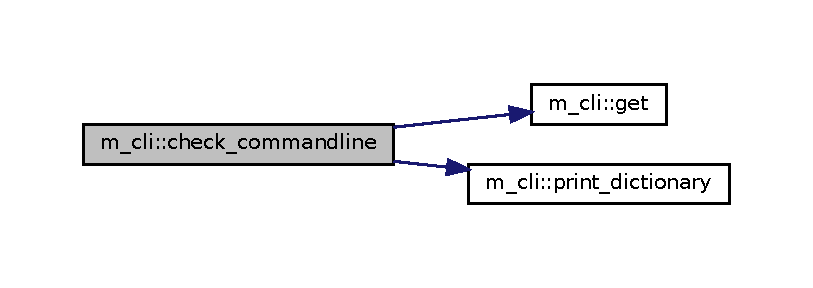
\includegraphics[width=350pt]{namespacem__cli_a62056f0c153eb63cb0b11a21edb028cd_cgraph}
\end{center}
\end{figure}
\mbox{\Hypertarget{namespacem__cli_a89a63254465b02048f09541e51974764}\label{namespacem__cli_a89a63254465b02048f09541e51974764}} 
\index{m\+\_\+cli@{m\+\_\+cli}!cmd\+\_\+args\+\_\+to\+\_\+dictionary@{cmd\+\_\+args\+\_\+to\+\_\+dictionary}}
\index{cmd\+\_\+args\+\_\+to\+\_\+dictionary@{cmd\+\_\+args\+\_\+to\+\_\+dictionary}!m\+\_\+cli@{m\+\_\+cli}}
\subsubsection{\texorpdfstring{cmd\+\_\+args\+\_\+to\+\_\+dictionary()}{cmd\_args\_to\_dictionary()}}
{\footnotesize\ttfamily subroutine m\+\_\+cli\+::cmd\+\_\+args\+\_\+to\+\_\+dictionary (\begin{DoxyParamCaption}\item[{logical, intent(in), optional}]{check }\end{DoxyParamCaption})\hspace{0.3cm}{\ttfamily [private]}}



References debug, g\+\_\+noquote, get(), ifnull(), keyword\+\_\+single, keywords, print\+\_\+dictionary(), quote(), substitute(), unnamed, update(), and upper().

Here is the call graph for this function\+:\nopagebreak
\begin{figure}[H]
\begin{center}
\leavevmode
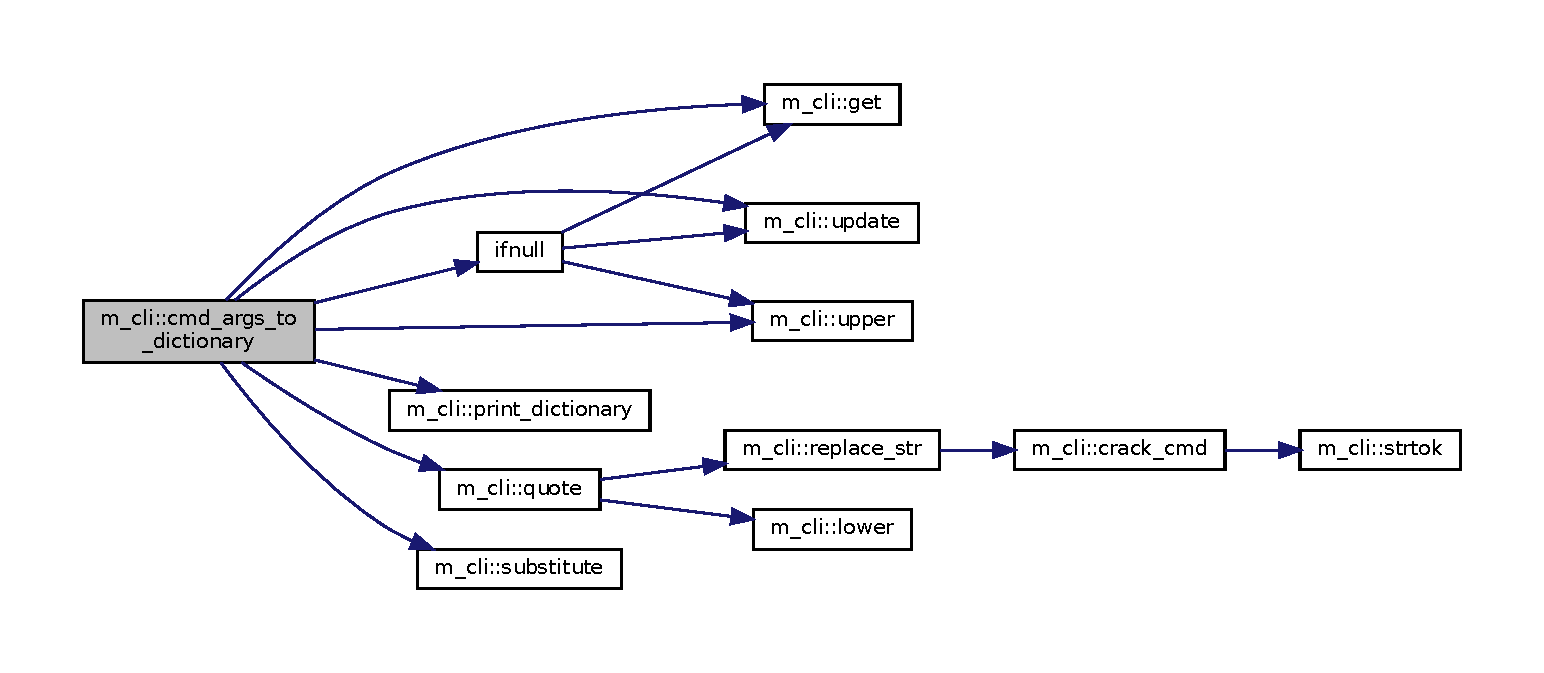
\includegraphics[width=350pt]{namespacem__cli_a89a63254465b02048f09541e51974764_cgraph}
\end{center}
\end{figure}
Here is the caller graph for this function\+:\nopagebreak
\begin{figure}[H]
\begin{center}
\leavevmode
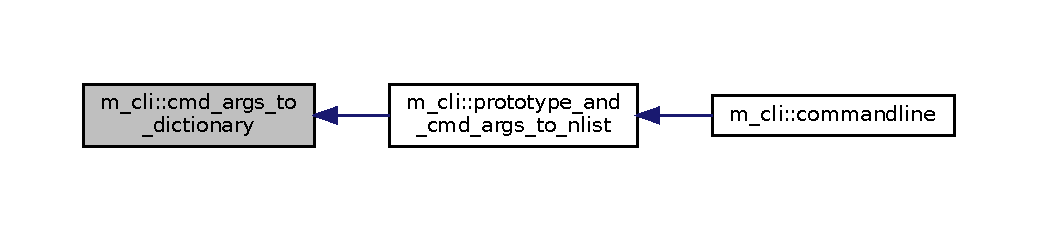
\includegraphics[width=350pt]{namespacem__cli_a89a63254465b02048f09541e51974764_icgraph}
\end{center}
\end{figure}
\mbox{\Hypertarget{namespacem__cli_a4f639b0c4bf16930fc1c5858ed4196a3}\label{namespacem__cli_a4f639b0c4bf16930fc1c5858ed4196a3}} 
\index{m\+\_\+cli@{m\+\_\+cli}!commandline@{commandline}}
\index{commandline@{commandline}!m\+\_\+cli@{m\+\_\+cli}}
\subsubsection{\texorpdfstring{commandline()}{commandline()}}
{\footnotesize\ttfamily character(len=\+:) function, allocatable, public m\+\_\+cli\+::commandline (\begin{DoxyParamCaption}\item[{character(len=$\ast$), intent(in)}]{definition,  }\item[{character(len=$\ast$), intent(in), optional}]{name,  }\item[{logical, optional}]{noquote }\end{DoxyParamCaption})}



References g\+\_\+namelist\+\_\+name, g\+\_\+noquote, longest\+\_\+command\+\_\+argument(), passed\+\_\+in, prototype\+\_\+and\+\_\+cmd\+\_\+args\+\_\+to\+\_\+nlist(), unnamed, and wipe\+\_\+dictionary().

Here is the call graph for this function\+:\nopagebreak
\begin{figure}[H]
\begin{center}
\leavevmode
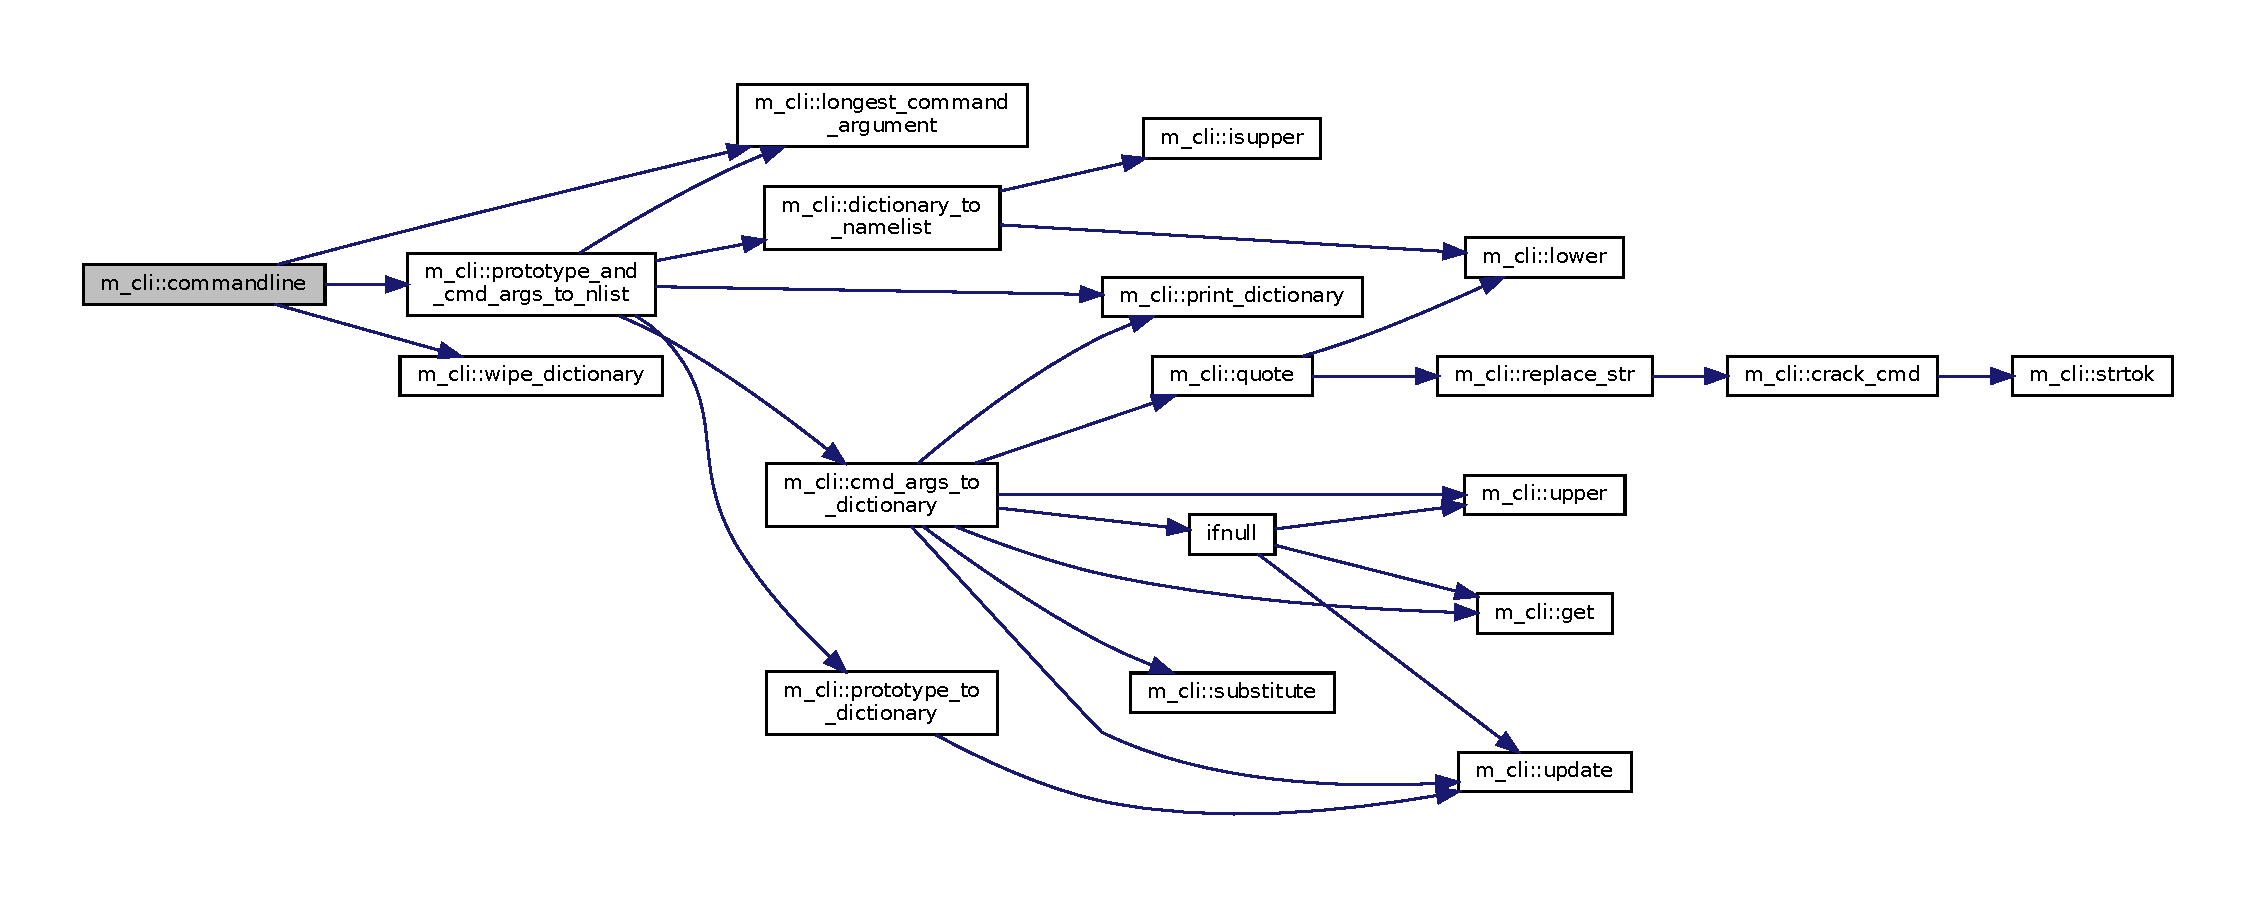
\includegraphics[width=350pt]{namespacem__cli_a4f639b0c4bf16930fc1c5858ed4196a3_cgraph}
\end{center}
\end{figure}
\mbox{\Hypertarget{namespacem__cli_a8d5d1954aac6494e07fb11f12f635c85}\label{namespacem__cli_a8d5d1954aac6494e07fb11f12f635c85}} 
\index{m\+\_\+cli@{m\+\_\+cli}!crack\+\_\+cmd@{crack\+\_\+cmd}}
\index{crack\+\_\+cmd@{crack\+\_\+cmd}!m\+\_\+cli@{m\+\_\+cli}}
\subsubsection{\texorpdfstring{crack\+\_\+cmd()}{crack\_cmd()}}
{\footnotesize\ttfamily subroutine m\+\_\+cli\+::crack\+\_\+cmd (\begin{DoxyParamCaption}\item[{character(len=$\ast$), intent(in)}]{cmd,  }\item[{character(len=\+:), intent(out), allocatable}]{old,  }\item[{character(len=\+:), intent(out), allocatable}]{new,  }\item[{integer}]{ierr }\end{DoxyParamCaption})\hspace{0.3cm}{\ttfamily [private]}}



References strtok().

Here is the call graph for this function\+:\nopagebreak
\begin{figure}[H]
\begin{center}
\leavevmode
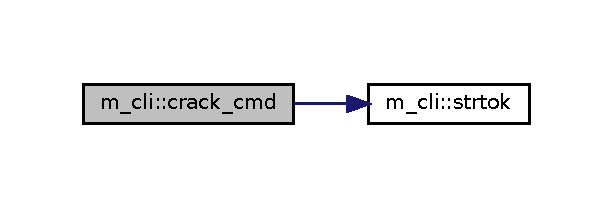
\includegraphics[width=294pt]{namespacem__cli_a8d5d1954aac6494e07fb11f12f635c85_cgraph}
\end{center}
\end{figure}
Here is the caller graph for this function\+:\nopagebreak
\begin{figure}[H]
\begin{center}
\leavevmode
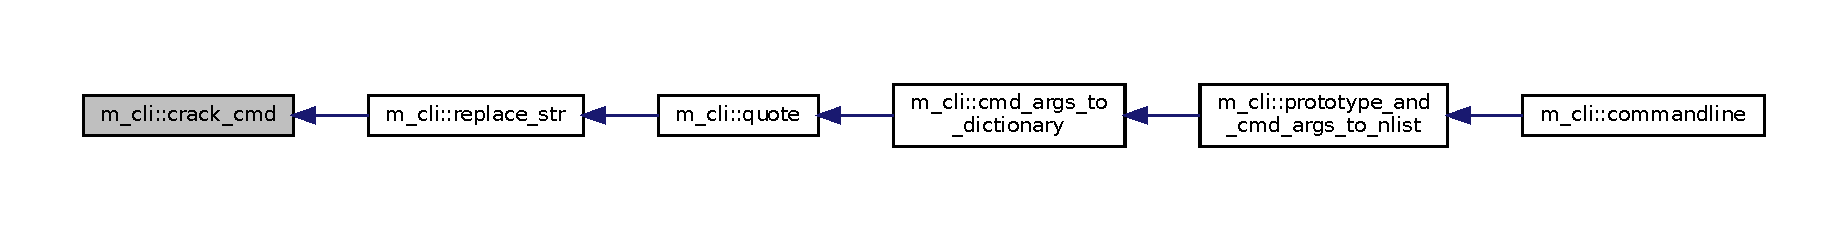
\includegraphics[width=350pt]{namespacem__cli_a8d5d1954aac6494e07fb11f12f635c85_icgraph}
\end{center}
\end{figure}
\mbox{\Hypertarget{namespacem__cli_a1be098e2b920e8d50ed14be03a3133db}\label{namespacem__cli_a1be098e2b920e8d50ed14be03a3133db}} 
\index{m\+\_\+cli@{m\+\_\+cli}!dict\+\_\+add@{dict\+\_\+add}}
\index{dict\+\_\+add@{dict\+\_\+add}!m\+\_\+cli@{m\+\_\+cli}}
\subsubsection{\texorpdfstring{dict\+\_\+add()}{dict\_add()}}
{\footnotesize\ttfamily subroutine m\+\_\+cli\+::dict\+\_\+add (\begin{DoxyParamCaption}\item[{class(\mbox{\hyperlink{structm__cli_1_1dictionary}{dictionary}}), intent(inout)}]{self,  }\item[{character(len=$\ast$), intent(in)}]{key,  }\item[{character(len=$\ast$), intent(in)}]{value }\end{DoxyParamCaption})\hspace{0.3cm}{\ttfamily [private]}}

\mbox{\Hypertarget{namespacem__cli_aff32e44070983c7fb4eb0a3b1dea7a6d}\label{namespacem__cli_aff32e44070983c7fb4eb0a3b1dea7a6d}} 
\index{m\+\_\+cli@{m\+\_\+cli}!dict\+\_\+delete@{dict\+\_\+delete}}
\index{dict\+\_\+delete@{dict\+\_\+delete}!m\+\_\+cli@{m\+\_\+cli}}
\subsubsection{\texorpdfstring{dict\+\_\+delete()}{dict\_delete()}}
{\footnotesize\ttfamily subroutine m\+\_\+cli\+::dict\+\_\+delete (\begin{DoxyParamCaption}\item[{class(\mbox{\hyperlink{structm__cli_1_1dictionary}{dictionary}}), intent(inout)}]{self,  }\item[{character(len=$\ast$), intent(in)}]{key }\end{DoxyParamCaption})\hspace{0.3cm}{\ttfamily [private]}}

\mbox{\Hypertarget{namespacem__cli_ac4a889309ffc333af6bf8e11f1fc4869}\label{namespacem__cli_ac4a889309ffc333af6bf8e11f1fc4869}} 
\index{m\+\_\+cli@{m\+\_\+cli}!dict\+\_\+get@{dict\+\_\+get}}
\index{dict\+\_\+get@{dict\+\_\+get}!m\+\_\+cli@{m\+\_\+cli}}
\subsubsection{\texorpdfstring{dict\+\_\+get()}{dict\_get()}}
{\footnotesize\ttfamily character(len=\+:) function, allocatable m\+\_\+cli\+::dict\+\_\+get (\begin{DoxyParamCaption}\item[{class(\mbox{\hyperlink{structm__cli_1_1dictionary}{dictionary}})}]{self,  }\item[{character(len=$\ast$), intent(in)}]{key }\end{DoxyParamCaption})\hspace{0.3cm}{\ttfamily [private]}}

\mbox{\Hypertarget{namespacem__cli_a7e5041efcad56387232475a3ae728634}\label{namespacem__cli_a7e5041efcad56387232475a3ae728634}} 
\index{m\+\_\+cli@{m\+\_\+cli}!dictionary\+\_\+to\+\_\+namelist@{dictionary\+\_\+to\+\_\+namelist}}
\index{dictionary\+\_\+to\+\_\+namelist@{dictionary\+\_\+to\+\_\+namelist}!m\+\_\+cli@{m\+\_\+cli}}
\subsubsection{\texorpdfstring{dictionary\+\_\+to\+\_\+namelist()}{dictionary\_to\_namelist()}}
{\footnotesize\ttfamily subroutine m\+\_\+cli\+::dictionary\+\_\+to\+\_\+namelist (\begin{DoxyParamCaption}\item[{character(len=\+:), intent(out), allocatable}]{nml }\end{DoxyParamCaption})\hspace{0.3cm}{\ttfamily [private]}}



References debug, isupper(), keywords, lower(), present\+\_\+in, return\+\_\+all, unnamed, and values.

Here is the call graph for this function\+:\nopagebreak
\begin{figure}[H]
\begin{center}
\leavevmode
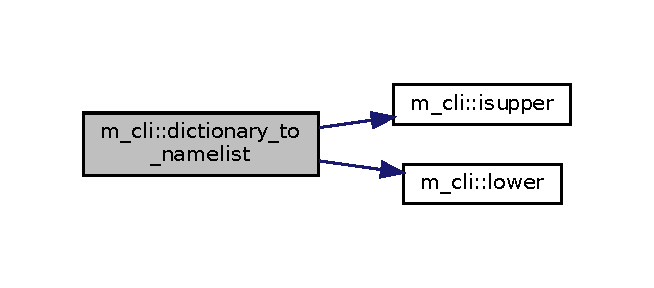
\includegraphics[width=314pt]{namespacem__cli_a7e5041efcad56387232475a3ae728634_cgraph}
\end{center}
\end{figure}
Here is the caller graph for this function\+:\nopagebreak
\begin{figure}[H]
\begin{center}
\leavevmode
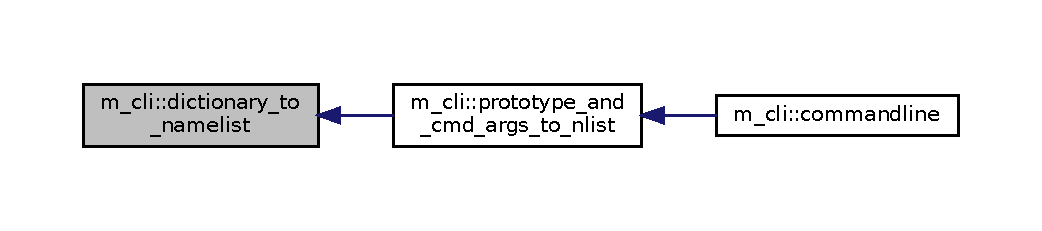
\includegraphics[width=350pt]{namespacem__cli_a7e5041efcad56387232475a3ae728634_icgraph}
\end{center}
\end{figure}
\mbox{\Hypertarget{namespacem__cli_a45783c194a1484042f63c58b180ca8df}\label{namespacem__cli_a45783c194a1484042f63c58b180ca8df}} 
\index{m\+\_\+cli@{m\+\_\+cli}!get@{get}}
\index{get@{get}!m\+\_\+cli@{m\+\_\+cli}}
\subsubsection{\texorpdfstring{get()}{get()}}
{\footnotesize\ttfamily character(len=\+:) function, allocatable, private m\+\_\+cli\+::get (\begin{DoxyParamCaption}\item[{character(len=$\ast$), intent(in)}]{key }\end{DoxyParamCaption})\hspace{0.3cm}{\ttfamily [private]}}



References counts, keywords, and values.

Here is the caller graph for this function\+:\nopagebreak
\begin{figure}[H]
\begin{center}
\leavevmode
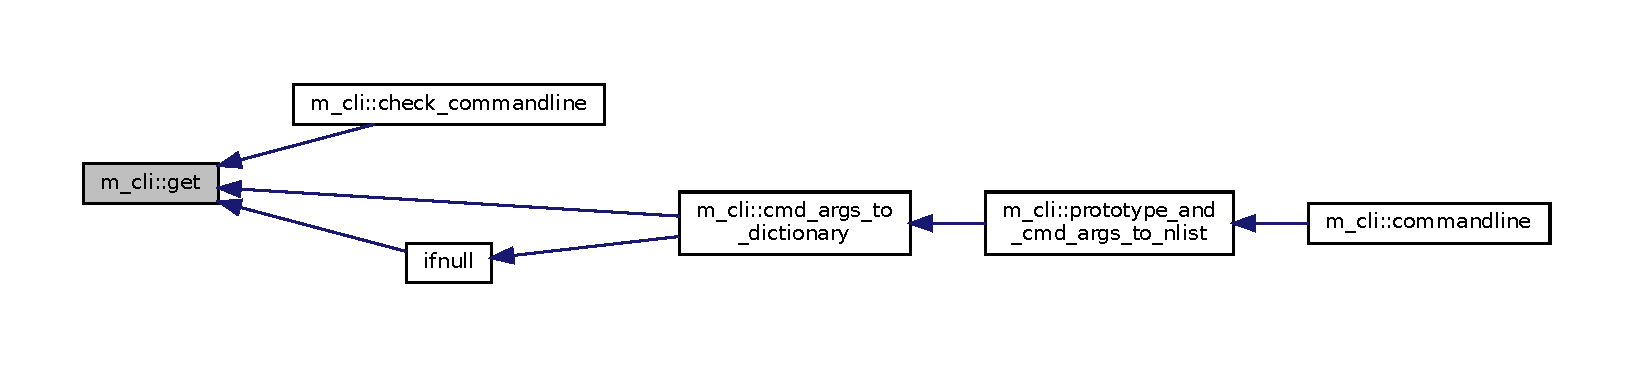
\includegraphics[width=350pt]{namespacem__cli_a45783c194a1484042f63c58b180ca8df_icgraph}
\end{center}
\end{figure}
\mbox{\Hypertarget{namespacem__cli_a9baf1cf0e20942fbde8c025ead5a30db}\label{namespacem__cli_a9baf1cf0e20942fbde8c025ead5a30db}} 
\index{m\+\_\+cli@{m\+\_\+cli}!insert\+\_\+c@{insert\+\_\+c}}
\index{insert\+\_\+c@{insert\+\_\+c}!m\+\_\+cli@{m\+\_\+cli}}
\subsubsection{\texorpdfstring{insert\+\_\+c()}{insert\_c()}}
{\footnotesize\ttfamily subroutine, private m\+\_\+cli\+::insert\+\_\+c (\begin{DoxyParamCaption}\item[{character(len=\+:), dimension(\+:), allocatable}]{list,  }\item[{character(len=$\ast$), intent(in)}]{value,  }\item[{integer, intent(in)}]{place }\end{DoxyParamCaption})\hspace{0.3cm}{\ttfamily [private]}}



References debug.

Here is the caller graph for this function\+:\nopagebreak
\begin{figure}[H]
\begin{center}
\leavevmode
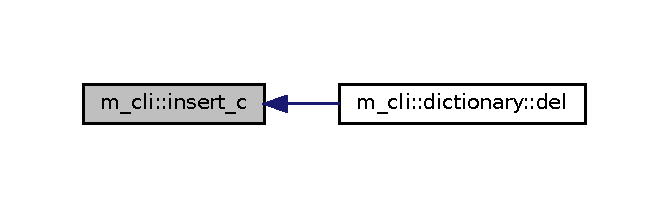
\includegraphics[width=321pt]{namespacem__cli_a9baf1cf0e20942fbde8c025ead5a30db_icgraph}
\end{center}
\end{figure}
\mbox{\Hypertarget{namespacem__cli_a030e31579a7968aea68d80db1e36ebfd}\label{namespacem__cli_a030e31579a7968aea68d80db1e36ebfd}} 
\index{m\+\_\+cli@{m\+\_\+cli}!insert\+\_\+d@{insert\+\_\+d}}
\index{insert\+\_\+d@{insert\+\_\+d}!m\+\_\+cli@{m\+\_\+cli}}
\subsubsection{\texorpdfstring{insert\+\_\+d()}{insert\_d()}}
{\footnotesize\ttfamily subroutine, private m\+\_\+cli\+::insert\+\_\+d (\begin{DoxyParamCaption}\item[{doubleprecision, dimension(\+:), allocatable}]{list,  }\item[{doubleprecision, intent(in)}]{value,  }\item[{integer, intent(in)}]{place }\end{DoxyParamCaption})\hspace{0.3cm}{\ttfamily [private]}}



References debug.

Here is the caller graph for this function\+:\nopagebreak
\begin{figure}[H]
\begin{center}
\leavevmode
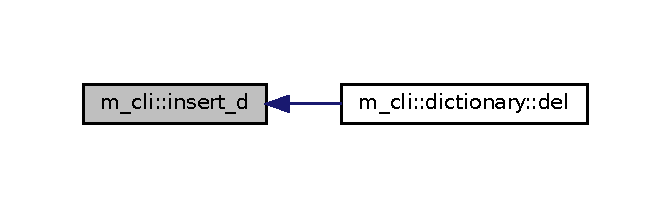
\includegraphics[width=322pt]{namespacem__cli_a030e31579a7968aea68d80db1e36ebfd_icgraph}
\end{center}
\end{figure}
\mbox{\Hypertarget{namespacem__cli_a841685591ef1f1827fc1fe32a7f546f1}\label{namespacem__cli_a841685591ef1f1827fc1fe32a7f546f1}} 
\index{m\+\_\+cli@{m\+\_\+cli}!insert\+\_\+i@{insert\+\_\+i}}
\index{insert\+\_\+i@{insert\+\_\+i}!m\+\_\+cli@{m\+\_\+cli}}
\subsubsection{\texorpdfstring{insert\+\_\+i()}{insert\_i()}}
{\footnotesize\ttfamily subroutine, private m\+\_\+cli\+::insert\+\_\+i (\begin{DoxyParamCaption}\item[{integer, dimension(\+:), allocatable}]{list,  }\item[{integer, intent(in)}]{value,  }\item[{integer, intent(in)}]{place }\end{DoxyParamCaption})\hspace{0.3cm}{\ttfamily [private]}}



References debug.

Here is the caller graph for this function\+:\nopagebreak
\begin{figure}[H]
\begin{center}
\leavevmode
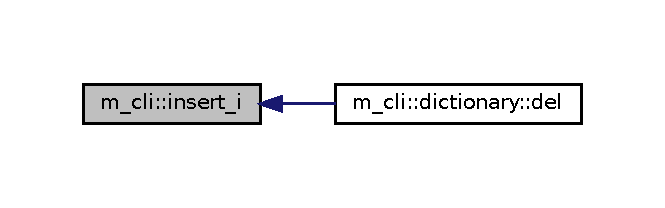
\includegraphics[width=319pt]{namespacem__cli_a841685591ef1f1827fc1fe32a7f546f1_icgraph}
\end{center}
\end{figure}
\mbox{\Hypertarget{namespacem__cli_a0c1b22c46470afbb4ee5c67180335578}\label{namespacem__cli_a0c1b22c46470afbb4ee5c67180335578}} 
\index{m\+\_\+cli@{m\+\_\+cli}!insert\+\_\+l@{insert\+\_\+l}}
\index{insert\+\_\+l@{insert\+\_\+l}!m\+\_\+cli@{m\+\_\+cli}}
\subsubsection{\texorpdfstring{insert\+\_\+l()}{insert\_l()}}
{\footnotesize\ttfamily subroutine, private m\+\_\+cli\+::insert\+\_\+l (\begin{DoxyParamCaption}\item[{logical, dimension(\+:), allocatable}]{list,  }\item[{logical, intent(in)}]{value,  }\item[{integer, intent(in)}]{place }\end{DoxyParamCaption})\hspace{0.3cm}{\ttfamily [private]}}



References debug.

Here is the caller graph for this function\+:\nopagebreak
\begin{figure}[H]
\begin{center}
\leavevmode
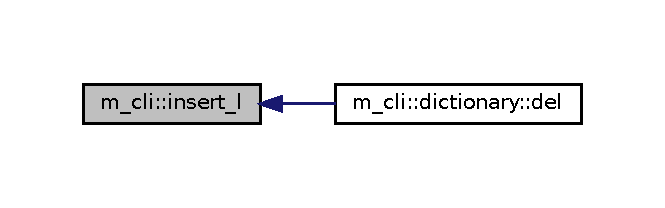
\includegraphics[width=319pt]{namespacem__cli_a0c1b22c46470afbb4ee5c67180335578_icgraph}
\end{center}
\end{figure}
\mbox{\Hypertarget{namespacem__cli_a4bfb90e14824f94017b1d4fcb39f0701}\label{namespacem__cli_a4bfb90e14824f94017b1d4fcb39f0701}} 
\index{m\+\_\+cli@{m\+\_\+cli}!insert\+\_\+r@{insert\+\_\+r}}
\index{insert\+\_\+r@{insert\+\_\+r}!m\+\_\+cli@{m\+\_\+cli}}
\subsubsection{\texorpdfstring{insert\+\_\+r()}{insert\_r()}}
{\footnotesize\ttfamily subroutine, private m\+\_\+cli\+::insert\+\_\+r (\begin{DoxyParamCaption}\item[{real, dimension(\+:), allocatable}]{list,  }\item[{real, intent(in)}]{value,  }\item[{integer, intent(in)}]{place }\end{DoxyParamCaption})\hspace{0.3cm}{\ttfamily [private]}}



References debug.

Here is the caller graph for this function\+:\nopagebreak
\begin{figure}[H]
\begin{center}
\leavevmode
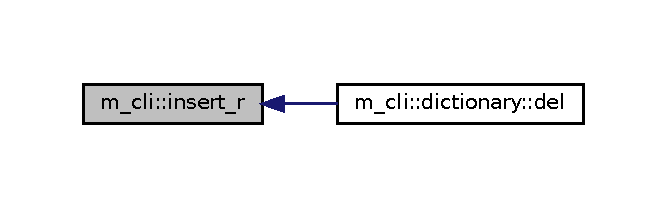
\includegraphics[width=320pt]{namespacem__cli_a4bfb90e14824f94017b1d4fcb39f0701_icgraph}
\end{center}
\end{figure}
\mbox{\Hypertarget{namespacem__cli_a4c126288dc18289b2095a0882f10ca77}\label{namespacem__cli_a4c126288dc18289b2095a0882f10ca77}} 
\index{m\+\_\+cli@{m\+\_\+cli}!isupper@{isupper}}
\index{isupper@{isupper}!m\+\_\+cli@{m\+\_\+cli}}
\subsubsection{\texorpdfstring{isupper()}{isupper()}}
{\footnotesize\ttfamily pure elemental logical function m\+\_\+cli\+::isupper (\begin{DoxyParamCaption}\item[{character, intent(in)}]{ch }\end{DoxyParamCaption})\hspace{0.3cm}{\ttfamily [private]}}

Here is the caller graph for this function\+:\nopagebreak
\begin{figure}[H]
\begin{center}
\leavevmode
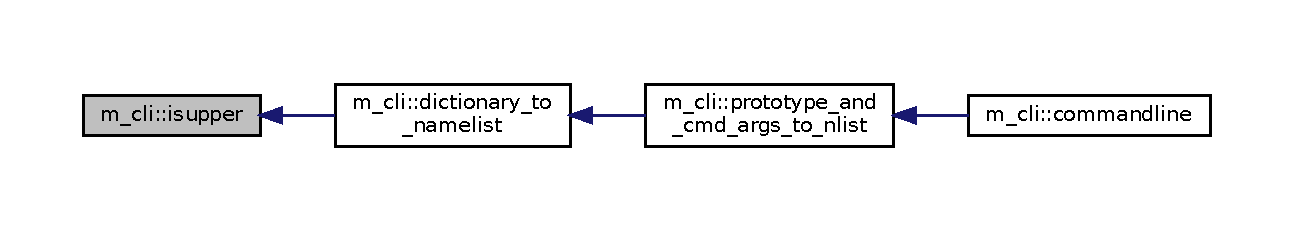
\includegraphics[width=350pt]{namespacem__cli_a4c126288dc18289b2095a0882f10ca77_icgraph}
\end{center}
\end{figure}
\mbox{\Hypertarget{namespacem__cli_ade3d1e36f0fc6a47b5469dcd8ade5312}\label{namespacem__cli_ade3d1e36f0fc6a47b5469dcd8ade5312}} 
\index{m\+\_\+cli@{m\+\_\+cli}!locate\+\_\+c@{locate\+\_\+c}}
\index{locate\+\_\+c@{locate\+\_\+c}!m\+\_\+cli@{m\+\_\+cli}}
\subsubsection{\texorpdfstring{locate\+\_\+c()}{locate\_c()}}
{\footnotesize\ttfamily subroutine, private m\+\_\+cli\+::locate\+\_\+c (\begin{DoxyParamCaption}\item[{character(len=\+:), dimension(\+:), allocatable}]{list,  }\item[{character(len=$\ast$), intent(in)}]{value,  }\item[{integer, intent(out)}]{place,  }\item[{integer, intent(out), optional}]{ier,  }\item[{character(len=$\ast$), intent(out), optional}]{errmsg }\end{DoxyParamCaption})\hspace{0.3cm}{\ttfamily [private]}}



References debug.

Here is the caller graph for this function\+:\nopagebreak
\begin{figure}[H]
\begin{center}
\leavevmode
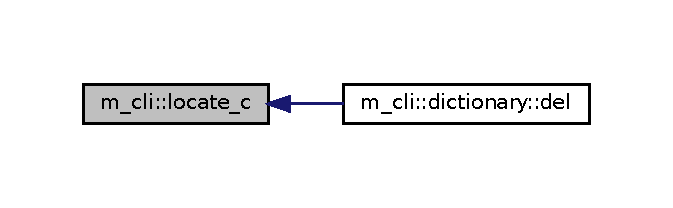
\includegraphics[width=323pt]{namespacem__cli_ade3d1e36f0fc6a47b5469dcd8ade5312_icgraph}
\end{center}
\end{figure}
\mbox{\Hypertarget{namespacem__cli_a4187c24a2abf5cc630232965637493e8}\label{namespacem__cli_a4187c24a2abf5cc630232965637493e8}} 
\index{m\+\_\+cli@{m\+\_\+cli}!locate\+\_\+d@{locate\+\_\+d}}
\index{locate\+\_\+d@{locate\+\_\+d}!m\+\_\+cli@{m\+\_\+cli}}
\subsubsection{\texorpdfstring{locate\+\_\+d()}{locate\_d()}}
{\footnotesize\ttfamily subroutine, private m\+\_\+cli\+::locate\+\_\+d (\begin{DoxyParamCaption}\item[{doubleprecision, dimension(\+:), allocatable}]{list,  }\item[{doubleprecision, intent(in)}]{value,  }\item[{integer, intent(out)}]{place,  }\item[{integer, intent(out), optional}]{ier,  }\item[{character(len=$\ast$), intent(out), optional}]{errmsg }\end{DoxyParamCaption})\hspace{0.3cm}{\ttfamily [private]}}



References debug.

Here is the caller graph for this function\+:\nopagebreak
\begin{figure}[H]
\begin{center}
\leavevmode
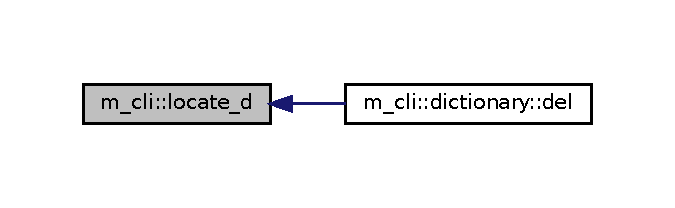
\includegraphics[width=324pt]{namespacem__cli_a4187c24a2abf5cc630232965637493e8_icgraph}
\end{center}
\end{figure}
\mbox{\Hypertarget{namespacem__cli_a36665ab0ea5080c14c8c9e52ed07d397}\label{namespacem__cli_a36665ab0ea5080c14c8c9e52ed07d397}} 
\index{m\+\_\+cli@{m\+\_\+cli}!locate\+\_\+i@{locate\+\_\+i}}
\index{locate\+\_\+i@{locate\+\_\+i}!m\+\_\+cli@{m\+\_\+cli}}
\subsubsection{\texorpdfstring{locate\+\_\+i()}{locate\_i()}}
{\footnotesize\ttfamily subroutine, private m\+\_\+cli\+::locate\+\_\+i (\begin{DoxyParamCaption}\item[{integer, dimension(\+:), allocatable}]{list,  }\item[{integer, intent(in)}]{value,  }\item[{integer, intent(out)}]{place,  }\item[{integer, intent(out), optional}]{ier,  }\item[{character(len=$\ast$), intent(out), optional}]{errmsg }\end{DoxyParamCaption})\hspace{0.3cm}{\ttfamily [private]}}



References debug.

Here is the caller graph for this function\+:\nopagebreak
\begin{figure}[H]
\begin{center}
\leavevmode
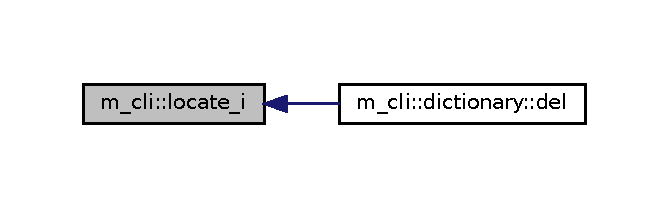
\includegraphics[width=321pt]{namespacem__cli_a36665ab0ea5080c14c8c9e52ed07d397_icgraph}
\end{center}
\end{figure}
\mbox{\Hypertarget{namespacem__cli_ac44389e115b536069f324bffea7d2469}\label{namespacem__cli_ac44389e115b536069f324bffea7d2469}} 
\index{m\+\_\+cli@{m\+\_\+cli}!locate\+\_\+r@{locate\+\_\+r}}
\index{locate\+\_\+r@{locate\+\_\+r}!m\+\_\+cli@{m\+\_\+cli}}
\subsubsection{\texorpdfstring{locate\+\_\+r()}{locate\_r()}}
{\footnotesize\ttfamily subroutine, private m\+\_\+cli\+::locate\+\_\+r (\begin{DoxyParamCaption}\item[{real, dimension(\+:), allocatable}]{list,  }\item[{real, intent(in)}]{value,  }\item[{integer, intent(out)}]{place,  }\item[{integer, intent(out), optional}]{ier,  }\item[{character(len=$\ast$), intent(out), optional}]{errmsg }\end{DoxyParamCaption})\hspace{0.3cm}{\ttfamily [private]}}



References debug.

Here is the caller graph for this function\+:\nopagebreak
\begin{figure}[H]
\begin{center}
\leavevmode
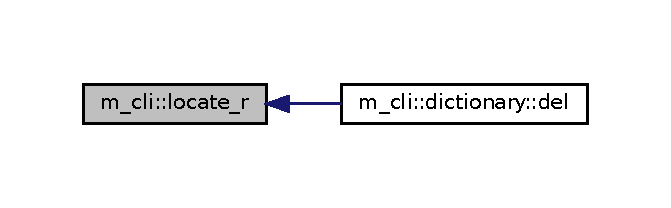
\includegraphics[width=322pt]{namespacem__cli_ac44389e115b536069f324bffea7d2469_icgraph}
\end{center}
\end{figure}
\mbox{\Hypertarget{namespacem__cli_aaf5504d3b48696a9d22fa5773c5a7d15}\label{namespacem__cli_aaf5504d3b48696a9d22fa5773c5a7d15}} 
\index{m\+\_\+cli@{m\+\_\+cli}!longest\+\_\+command\+\_\+argument@{longest\+\_\+command\+\_\+argument}}
\index{longest\+\_\+command\+\_\+argument@{longest\+\_\+command\+\_\+argument}!m\+\_\+cli@{m\+\_\+cli}}
\subsubsection{\texorpdfstring{longest\+\_\+command\+\_\+argument()}{longest\_command\_argument()}}
{\footnotesize\ttfamily integer function, private m\+\_\+cli\+::longest\+\_\+command\+\_\+argument (\begin{DoxyParamCaption}{ }\end{DoxyParamCaption})\hspace{0.3cm}{\ttfamily [private]}}

Here is the caller graph for this function\+:\nopagebreak
\begin{figure}[H]
\begin{center}
\leavevmode
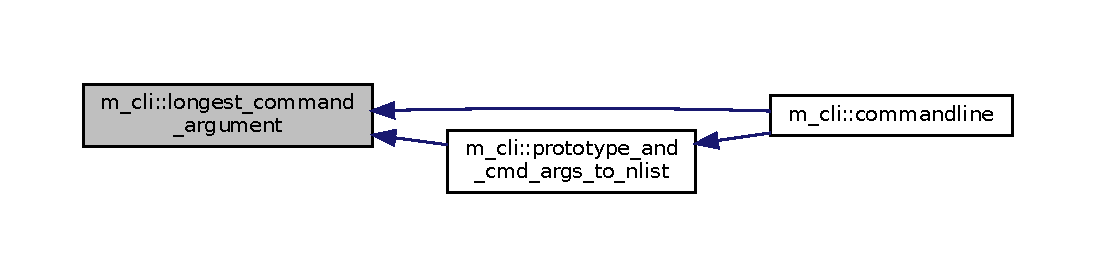
\includegraphics[width=350pt]{namespacem__cli_aaf5504d3b48696a9d22fa5773c5a7d15_icgraph}
\end{center}
\end{figure}
\mbox{\Hypertarget{namespacem__cli_a685574282a09c3f57e0c18654a3a642c}\label{namespacem__cli_a685574282a09c3f57e0c18654a3a642c}} 
\index{m\+\_\+cli@{m\+\_\+cli}!lower@{lower}}
\index{lower@{lower}!m\+\_\+cli@{m\+\_\+cli}}
\subsubsection{\texorpdfstring{lower()}{lower()}}
{\footnotesize\ttfamily elemental pure character(len(str)) function m\+\_\+cli\+::lower (\begin{DoxyParamCaption}\item[{character($\ast$), intent(in)}]{str,  }\item[{integer, intent(in), optional}]{begin,  }\item[{integer, intent(in), optional}]{end }\end{DoxyParamCaption})\hspace{0.3cm}{\ttfamily [private]}}

Here is the caller graph for this function\+:\nopagebreak
\begin{figure}[H]
\begin{center}
\leavevmode
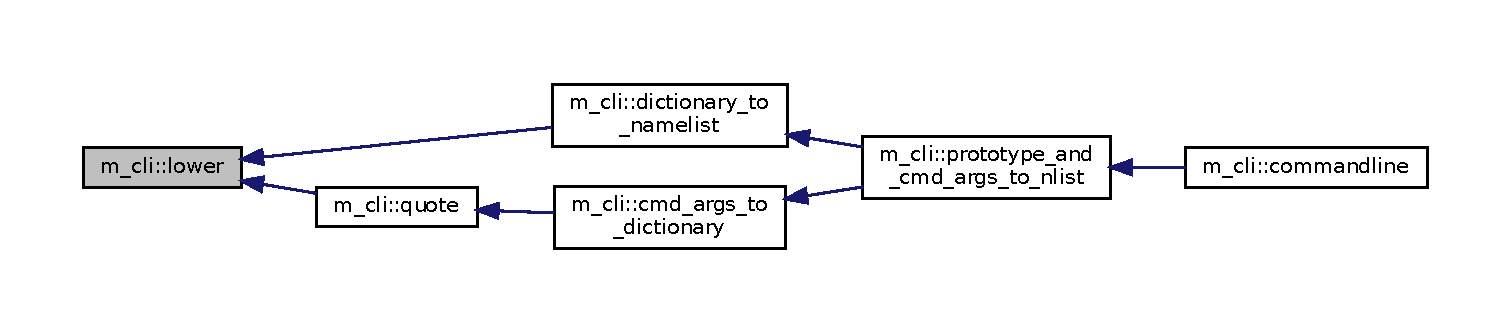
\includegraphics[width=350pt]{namespacem__cli_a685574282a09c3f57e0c18654a3a642c_icgraph}
\end{center}
\end{figure}
\mbox{\Hypertarget{namespacem__cli_a5b6abaf1d5aec5e918be0759df29c849}\label{namespacem__cli_a5b6abaf1d5aec5e918be0759df29c849}} 
\index{m\+\_\+cli@{m\+\_\+cli}!print\+\_\+dictionary@{print\+\_\+dictionary}}
\index{print\+\_\+dictionary@{print\+\_\+dictionary}!m\+\_\+cli@{m\+\_\+cli}}
\subsubsection{\texorpdfstring{print\+\_\+dictionary()}{print\_dictionary()}}
{\footnotesize\ttfamily subroutine, public m\+\_\+cli\+::print\+\_\+dictionary (\begin{DoxyParamCaption}\item[{character(len=$\ast$), intent(in), optional}]{header,  }\item[{logical, intent(in), optional}]{stop }\end{DoxyParamCaption})}



References counts, keywords, present\+\_\+in, unnamed, and values.

Here is the caller graph for this function\+:\nopagebreak
\begin{figure}[H]
\begin{center}
\leavevmode
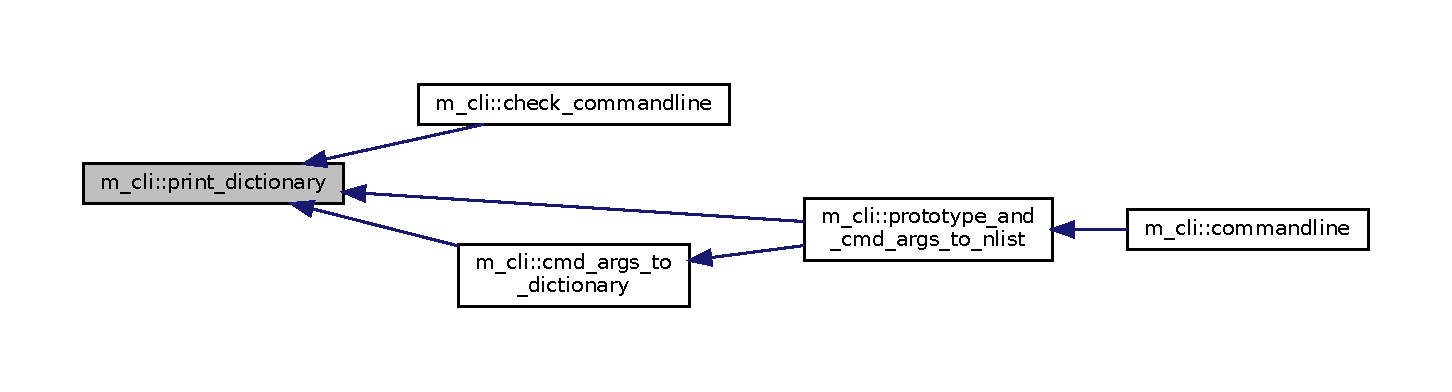
\includegraphics[width=350pt]{namespacem__cli_a5b6abaf1d5aec5e918be0759df29c849_icgraph}
\end{center}
\end{figure}
\mbox{\Hypertarget{namespacem__cli_ac77d70573b34ade2079cc4004a6acba5}\label{namespacem__cli_ac77d70573b34ade2079cc4004a6acba5}} 
\index{m\+\_\+cli@{m\+\_\+cli}!prototype\+\_\+and\+\_\+cmd\+\_\+args\+\_\+to\+\_\+nlist@{prototype\+\_\+and\+\_\+cmd\+\_\+args\+\_\+to\+\_\+nlist}}
\index{prototype\+\_\+and\+\_\+cmd\+\_\+args\+\_\+to\+\_\+nlist@{prototype\+\_\+and\+\_\+cmd\+\_\+args\+\_\+to\+\_\+nlist}!m\+\_\+cli@{m\+\_\+cli}}
\subsubsection{\texorpdfstring{prototype\+\_\+and\+\_\+cmd\+\_\+args\+\_\+to\+\_\+nlist()}{prototype\_and\_cmd\_args\_to\_nlist()}}
{\footnotesize\ttfamily subroutine, private m\+\_\+cli\+::prototype\+\_\+and\+\_\+cmd\+\_\+args\+\_\+to\+\_\+nlist (\begin{DoxyParamCaption}\item[{character(len=$\ast$), intent(in)}]{prototype,  }\item[{character(len=\+:), intent(out), allocatable}]{nml }\end{DoxyParamCaption})\hspace{0.3cm}{\ttfamily [private]}}



References cmd\+\_\+args\+\_\+to\+\_\+dictionary(), debug, dictionary\+\_\+to\+\_\+namelist(), g\+\_\+namelist\+\_\+name, longest\+\_\+command\+\_\+argument(), passed\+\_\+in, present\+\_\+in, print\+\_\+dictionary(), prototype\+\_\+to\+\_\+dictionary(), return\+\_\+all, and unnamed.

Here is the call graph for this function\+:\nopagebreak
\begin{figure}[H]
\begin{center}
\leavevmode
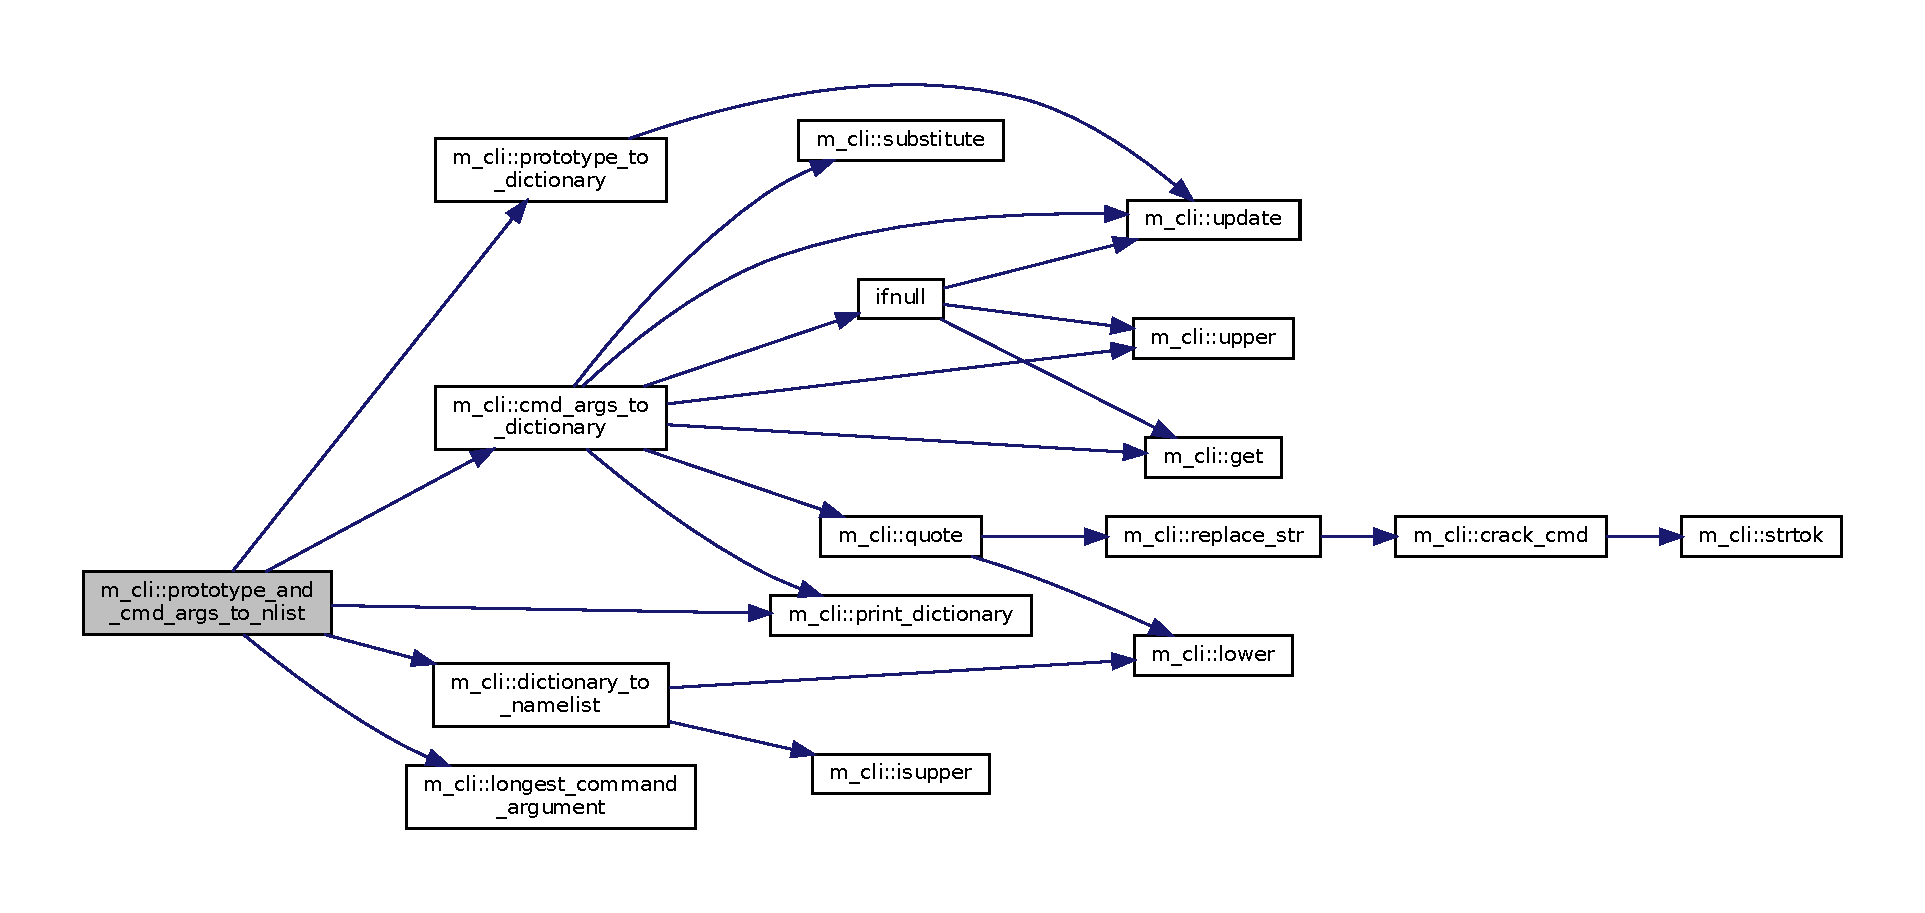
\includegraphics[width=350pt]{namespacem__cli_ac77d70573b34ade2079cc4004a6acba5_cgraph}
\end{center}
\end{figure}
Here is the caller graph for this function\+:\nopagebreak
\begin{figure}[H]
\begin{center}
\leavevmode
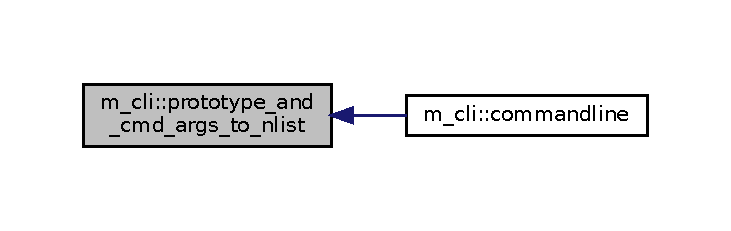
\includegraphics[width=350pt]{namespacem__cli_ac77d70573b34ade2079cc4004a6acba5_icgraph}
\end{center}
\end{figure}
\mbox{\Hypertarget{namespacem__cli_a8c62537a2d224364c9cb30005be819e9}\label{namespacem__cli_a8c62537a2d224364c9cb30005be819e9}} 
\index{m\+\_\+cli@{m\+\_\+cli}!prototype\+\_\+to\+\_\+dictionary@{prototype\+\_\+to\+\_\+dictionary}}
\index{prototype\+\_\+to\+\_\+dictionary@{prototype\+\_\+to\+\_\+dictionary}!m\+\_\+cli@{m\+\_\+cli}}
\subsubsection{\texorpdfstring{prototype\+\_\+to\+\_\+dictionary()}{prototype\_to\_dictionary()}}
{\footnotesize\ttfamily subroutine, private m\+\_\+cli\+::prototype\+\_\+to\+\_\+dictionary (\begin{DoxyParamCaption}\item[{character(len=$\ast$), intent(in)}]{string }\end{DoxyParamCaption})\hspace{0.3cm}{\ttfamily [private]}}



References debug, keyword\+\_\+single, and update().

Here is the call graph for this function\+:\nopagebreak
\begin{figure}[H]
\begin{center}
\leavevmode
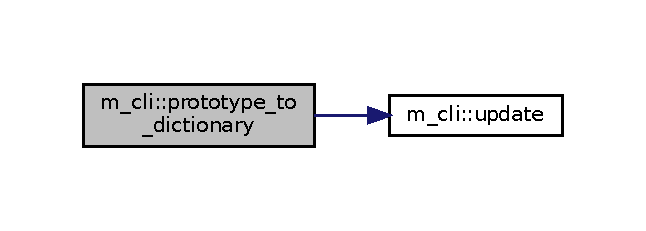
\includegraphics[width=310pt]{namespacem__cli_a8c62537a2d224364c9cb30005be819e9_cgraph}
\end{center}
\end{figure}
Here is the caller graph for this function\+:\nopagebreak
\begin{figure}[H]
\begin{center}
\leavevmode
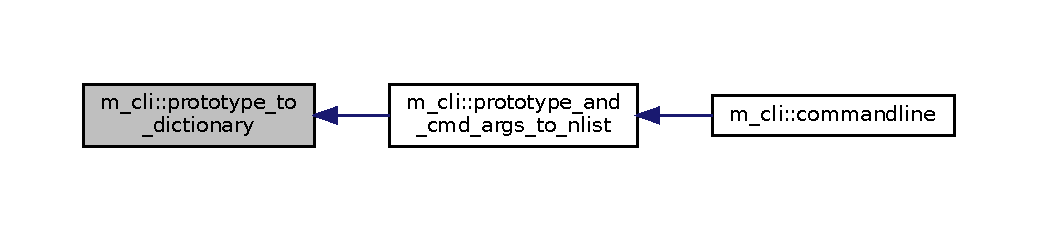
\includegraphics[width=350pt]{namespacem__cli_a8c62537a2d224364c9cb30005be819e9_icgraph}
\end{center}
\end{figure}
\mbox{\Hypertarget{namespacem__cli_ac82fec2a5441020701fe3c64af3d9948}\label{namespacem__cli_ac82fec2a5441020701fe3c64af3d9948}} 
\index{m\+\_\+cli@{m\+\_\+cli}!quote@{quote}}
\index{quote@{quote}!m\+\_\+cli@{m\+\_\+cli}}
\subsubsection{\texorpdfstring{quote()}{quote()}}
{\footnotesize\ttfamily character(len=\+:) function, allocatable m\+\_\+cli\+::quote (\begin{DoxyParamCaption}\item[{character(len=$\ast$), intent(in)}]{str,  }\item[{character(len=$\ast$), intent(in), optional}]{mode }\end{DoxyParamCaption})\hspace{0.3cm}{\ttfamily [private]}}



References lower(), and replace\+\_\+str().

Here is the call graph for this function\+:\nopagebreak
\begin{figure}[H]
\begin{center}
\leavevmode
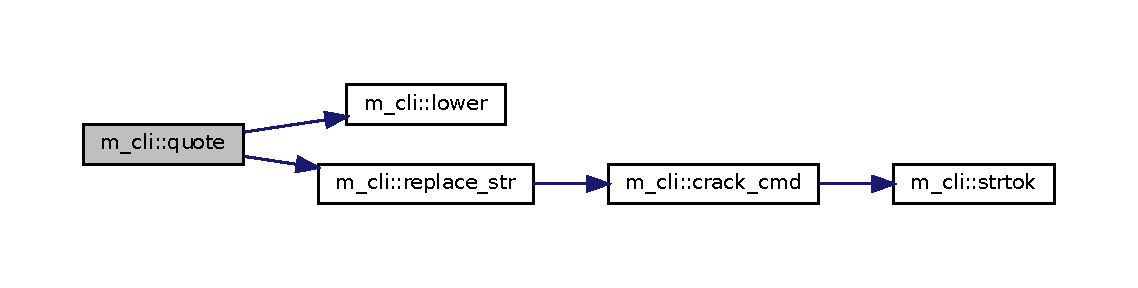
\includegraphics[width=350pt]{namespacem__cli_ac82fec2a5441020701fe3c64af3d9948_cgraph}
\end{center}
\end{figure}
Here is the caller graph for this function\+:\nopagebreak
\begin{figure}[H]
\begin{center}
\leavevmode
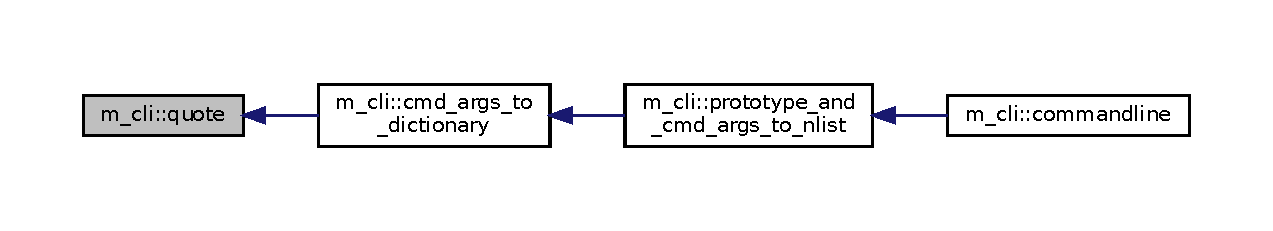
\includegraphics[width=350pt]{namespacem__cli_ac82fec2a5441020701fe3c64af3d9948_icgraph}
\end{center}
\end{figure}
\mbox{\Hypertarget{namespacem__cli_a05f549b10f50798d68003b8fd2a2d86a}\label{namespacem__cli_a05f549b10f50798d68003b8fd2a2d86a}} 
\index{m\+\_\+cli@{m\+\_\+cli}!remove\+\_\+c@{remove\+\_\+c}}
\index{remove\+\_\+c@{remove\+\_\+c}!m\+\_\+cli@{m\+\_\+cli}}
\subsubsection{\texorpdfstring{remove\+\_\+c()}{remove\_c()}}
{\footnotesize\ttfamily subroutine, private m\+\_\+cli\+::remove\+\_\+c (\begin{DoxyParamCaption}\item[{character(len=\+:), dimension(\+:), allocatable}]{list,  }\item[{integer, intent(in)}]{place }\end{DoxyParamCaption})\hspace{0.3cm}{\ttfamily [private]}}



References debug.

Here is the caller graph for this function\+:\nopagebreak
\begin{figure}[H]
\begin{center}
\leavevmode
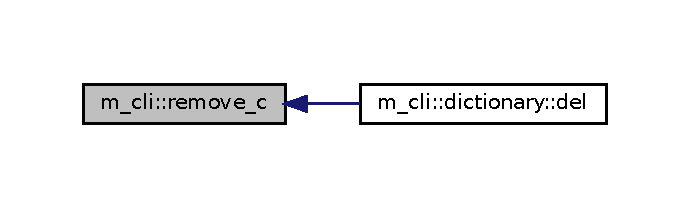
\includegraphics[width=331pt]{namespacem__cli_a05f549b10f50798d68003b8fd2a2d86a_icgraph}
\end{center}
\end{figure}
\mbox{\Hypertarget{namespacem__cli_abf22cbc2af66482f33b7bb1a210d9d99}\label{namespacem__cli_abf22cbc2af66482f33b7bb1a210d9d99}} 
\index{m\+\_\+cli@{m\+\_\+cli}!remove\+\_\+d@{remove\+\_\+d}}
\index{remove\+\_\+d@{remove\+\_\+d}!m\+\_\+cli@{m\+\_\+cli}}
\subsubsection{\texorpdfstring{remove\+\_\+d()}{remove\_d()}}
{\footnotesize\ttfamily subroutine, private m\+\_\+cli\+::remove\+\_\+d (\begin{DoxyParamCaption}\item[{doubleprecision, dimension(\+:), allocatable}]{list,  }\item[{integer, intent(in)}]{place }\end{DoxyParamCaption})\hspace{0.3cm}{\ttfamily [private]}}



References debug.

Here is the caller graph for this function\+:\nopagebreak
\begin{figure}[H]
\begin{center}
\leavevmode
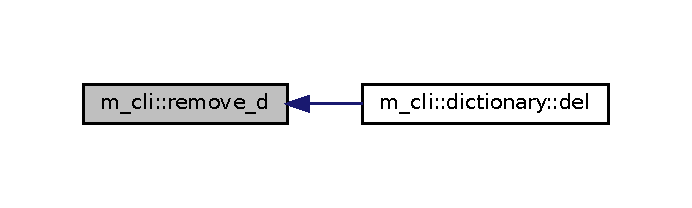
\includegraphics[width=332pt]{namespacem__cli_abf22cbc2af66482f33b7bb1a210d9d99_icgraph}
\end{center}
\end{figure}
\mbox{\Hypertarget{namespacem__cli_afa08d3d87184a6dd68a124231e536c93}\label{namespacem__cli_afa08d3d87184a6dd68a124231e536c93}} 
\index{m\+\_\+cli@{m\+\_\+cli}!remove\+\_\+i@{remove\+\_\+i}}
\index{remove\+\_\+i@{remove\+\_\+i}!m\+\_\+cli@{m\+\_\+cli}}
\subsubsection{\texorpdfstring{remove\+\_\+i()}{remove\_i()}}
{\footnotesize\ttfamily subroutine, private m\+\_\+cli\+::remove\+\_\+i (\begin{DoxyParamCaption}\item[{integer, dimension(\+:), allocatable}]{list,  }\item[{integer, intent(in)}]{place }\end{DoxyParamCaption})\hspace{0.3cm}{\ttfamily [private]}}



References debug.

Here is the caller graph for this function\+:\nopagebreak
\begin{figure}[H]
\begin{center}
\leavevmode
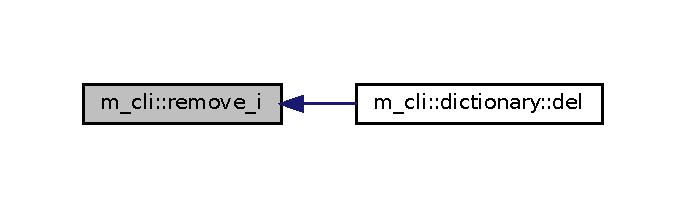
\includegraphics[width=329pt]{namespacem__cli_afa08d3d87184a6dd68a124231e536c93_icgraph}
\end{center}
\end{figure}
\mbox{\Hypertarget{namespacem__cli_a9c86f0f52ce71f14e774fd21f0686cf6}\label{namespacem__cli_a9c86f0f52ce71f14e774fd21f0686cf6}} 
\index{m\+\_\+cli@{m\+\_\+cli}!remove\+\_\+l@{remove\+\_\+l}}
\index{remove\+\_\+l@{remove\+\_\+l}!m\+\_\+cli@{m\+\_\+cli}}
\subsubsection{\texorpdfstring{remove\+\_\+l()}{remove\_l()}}
{\footnotesize\ttfamily subroutine, private m\+\_\+cli\+::remove\+\_\+l (\begin{DoxyParamCaption}\item[{logical, dimension(\+:), allocatable}]{list,  }\item[{integer, intent(in)}]{place }\end{DoxyParamCaption})\hspace{0.3cm}{\ttfamily [private]}}



References debug.

Here is the caller graph for this function\+:\nopagebreak
\begin{figure}[H]
\begin{center}
\leavevmode
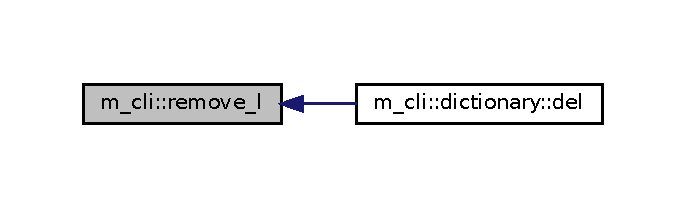
\includegraphics[width=329pt]{namespacem__cli_a9c86f0f52ce71f14e774fd21f0686cf6_icgraph}
\end{center}
\end{figure}
\mbox{\Hypertarget{namespacem__cli_a4f47701695b95c88fa4927c04996ce0f}\label{namespacem__cli_a4f47701695b95c88fa4927c04996ce0f}} 
\index{m\+\_\+cli@{m\+\_\+cli}!remove\+\_\+r@{remove\+\_\+r}}
\index{remove\+\_\+r@{remove\+\_\+r}!m\+\_\+cli@{m\+\_\+cli}}
\subsubsection{\texorpdfstring{remove\+\_\+r()}{remove\_r()}}
{\footnotesize\ttfamily subroutine, private m\+\_\+cli\+::remove\+\_\+r (\begin{DoxyParamCaption}\item[{real, dimension(\+:), allocatable}]{list,  }\item[{integer, intent(in)}]{place }\end{DoxyParamCaption})\hspace{0.3cm}{\ttfamily [private]}}



References debug.

Here is the caller graph for this function\+:\nopagebreak
\begin{figure}[H]
\begin{center}
\leavevmode
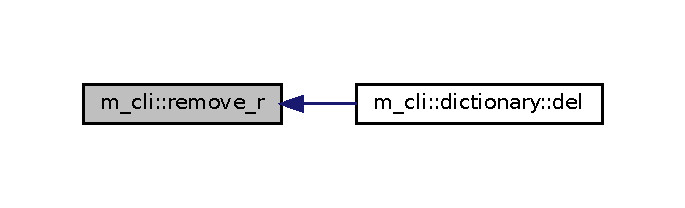
\includegraphics[width=329pt]{namespacem__cli_a4f47701695b95c88fa4927c04996ce0f_icgraph}
\end{center}
\end{figure}
\mbox{\Hypertarget{namespacem__cli_a785aa0016768b6dc2e27c29d5342c329}\label{namespacem__cli_a785aa0016768b6dc2e27c29d5342c329}} 
\index{m\+\_\+cli@{m\+\_\+cli}!replace\+\_\+c@{replace\+\_\+c}}
\index{replace\+\_\+c@{replace\+\_\+c}!m\+\_\+cli@{m\+\_\+cli}}
\subsubsection{\texorpdfstring{replace\+\_\+c()}{replace\_c()}}
{\footnotesize\ttfamily subroutine, private m\+\_\+cli\+::replace\+\_\+c (\begin{DoxyParamCaption}\item[{character(len=\+:), dimension(\+:), allocatable}]{list,  }\item[{character(len=$\ast$), intent(in)}]{value,  }\item[{integer, intent(in)}]{place }\end{DoxyParamCaption})\hspace{0.3cm}{\ttfamily [private]}}



References debug.

Here is the caller graph for this function\+:\nopagebreak
\begin{figure}[H]
\begin{center}
\leavevmode
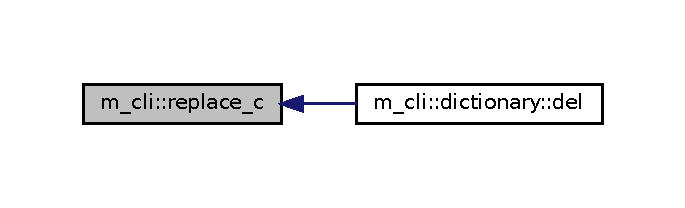
\includegraphics[width=329pt]{namespacem__cli_a785aa0016768b6dc2e27c29d5342c329_icgraph}
\end{center}
\end{figure}
\mbox{\Hypertarget{namespacem__cli_aa9b7d672cc9fb0bc79fd09a2870614f5}\label{namespacem__cli_aa9b7d672cc9fb0bc79fd09a2870614f5}} 
\index{m\+\_\+cli@{m\+\_\+cli}!replace\+\_\+d@{replace\+\_\+d}}
\index{replace\+\_\+d@{replace\+\_\+d}!m\+\_\+cli@{m\+\_\+cli}}
\subsubsection{\texorpdfstring{replace\+\_\+d()}{replace\_d()}}
{\footnotesize\ttfamily subroutine, private m\+\_\+cli\+::replace\+\_\+d (\begin{DoxyParamCaption}\item[{doubleprecision, dimension(\+:), allocatable}]{list,  }\item[{doubleprecision, intent(in)}]{value,  }\item[{integer, intent(in)}]{place }\end{DoxyParamCaption})\hspace{0.3cm}{\ttfamily [private]}}



References debug.

Here is the caller graph for this function\+:\nopagebreak
\begin{figure}[H]
\begin{center}
\leavevmode
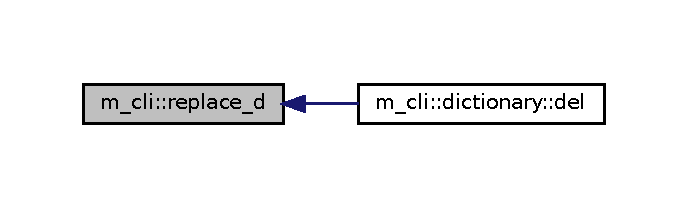
\includegraphics[width=330pt]{namespacem__cli_aa9b7d672cc9fb0bc79fd09a2870614f5_icgraph}
\end{center}
\end{figure}
\mbox{\Hypertarget{namespacem__cli_ac609c48bb1f904235b8cbf8bea61473f}\label{namespacem__cli_ac609c48bb1f904235b8cbf8bea61473f}} 
\index{m\+\_\+cli@{m\+\_\+cli}!replace\+\_\+i@{replace\+\_\+i}}
\index{replace\+\_\+i@{replace\+\_\+i}!m\+\_\+cli@{m\+\_\+cli}}
\subsubsection{\texorpdfstring{replace\+\_\+i()}{replace\_i()}}
{\footnotesize\ttfamily subroutine, private m\+\_\+cli\+::replace\+\_\+i (\begin{DoxyParamCaption}\item[{integer, dimension(\+:), allocatable}]{list,  }\item[{integer, intent(in)}]{value,  }\item[{integer, intent(in)}]{place }\end{DoxyParamCaption})\hspace{0.3cm}{\ttfamily [private]}}



References debug.

Here is the caller graph for this function\+:\nopagebreak
\begin{figure}[H]
\begin{center}
\leavevmode
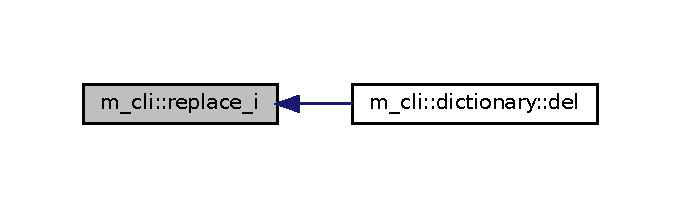
\includegraphics[width=327pt]{namespacem__cli_ac609c48bb1f904235b8cbf8bea61473f_icgraph}
\end{center}
\end{figure}
\mbox{\Hypertarget{namespacem__cli_a89ed5c3b944f91d8135173206fbc7e07}\label{namespacem__cli_a89ed5c3b944f91d8135173206fbc7e07}} 
\index{m\+\_\+cli@{m\+\_\+cli}!replace\+\_\+l@{replace\+\_\+l}}
\index{replace\+\_\+l@{replace\+\_\+l}!m\+\_\+cli@{m\+\_\+cli}}
\subsubsection{\texorpdfstring{replace\+\_\+l()}{replace\_l()}}
{\footnotesize\ttfamily subroutine, private m\+\_\+cli\+::replace\+\_\+l (\begin{DoxyParamCaption}\item[{logical, dimension(\+:), allocatable}]{list,  }\item[{logical, intent(in)}]{value,  }\item[{integer, intent(in)}]{place }\end{DoxyParamCaption})\hspace{0.3cm}{\ttfamily [private]}}



References debug.

Here is the caller graph for this function\+:\nopagebreak
\begin{figure}[H]
\begin{center}
\leavevmode
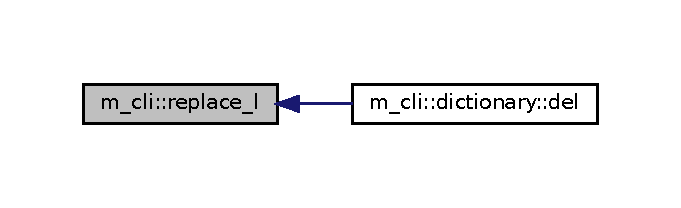
\includegraphics[width=327pt]{namespacem__cli_a89ed5c3b944f91d8135173206fbc7e07_icgraph}
\end{center}
\end{figure}
\mbox{\Hypertarget{namespacem__cli_ab3b33abc8a6da174d3f27c2f2203038c}\label{namespacem__cli_ab3b33abc8a6da174d3f27c2f2203038c}} 
\index{m\+\_\+cli@{m\+\_\+cli}!replace\+\_\+r@{replace\+\_\+r}}
\index{replace\+\_\+r@{replace\+\_\+r}!m\+\_\+cli@{m\+\_\+cli}}
\subsubsection{\texorpdfstring{replace\+\_\+r()}{replace\_r()}}
{\footnotesize\ttfamily subroutine, private m\+\_\+cli\+::replace\+\_\+r (\begin{DoxyParamCaption}\item[{real, dimension(\+:), allocatable}]{list,  }\item[{real, intent(in)}]{value,  }\item[{integer, intent(in)}]{place }\end{DoxyParamCaption})\hspace{0.3cm}{\ttfamily [private]}}



References debug.

Here is the caller graph for this function\+:\nopagebreak
\begin{figure}[H]
\begin{center}
\leavevmode
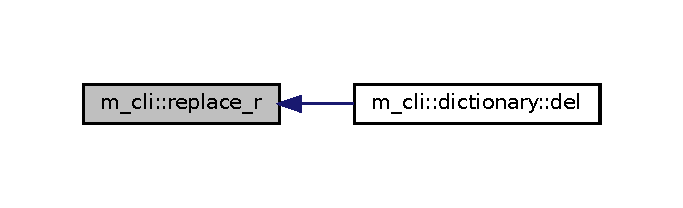
\includegraphics[width=328pt]{namespacem__cli_ab3b33abc8a6da174d3f27c2f2203038c_icgraph}
\end{center}
\end{figure}
\mbox{\Hypertarget{namespacem__cli_a40e02b1c9fc580ddd410bb24017fab8c}\label{namespacem__cli_a40e02b1c9fc580ddd410bb24017fab8c}} 
\index{m\+\_\+cli@{m\+\_\+cli}!replace\+\_\+str@{replace\+\_\+str}}
\index{replace\+\_\+str@{replace\+\_\+str}!m\+\_\+cli@{m\+\_\+cli}}
\subsubsection{\texorpdfstring{replace\+\_\+str()}{replace\_str()}}
{\footnotesize\ttfamily character(len=\+:) function, allocatable m\+\_\+cli\+::replace\+\_\+str (\begin{DoxyParamCaption}\item[{character(len=$\ast$), intent(in)}]{targetline,  }\item[{character(len=$\ast$), intent(in), optional}]{old,  }\item[{character(len=$\ast$), intent(in), optional}]{new,  }\item[{integer, intent(out), optional}]{ierr,  }\item[{character(len=$\ast$), intent(in), optional}]{cmd,  }\item[{integer, dimension(2), intent(in), optional}]{range }\end{DoxyParamCaption})\hspace{0.3cm}{\ttfamily [private]}}



References crack\+\_\+cmd().

Here is the call graph for this function\+:\nopagebreak
\begin{figure}[H]
\begin{center}
\leavevmode
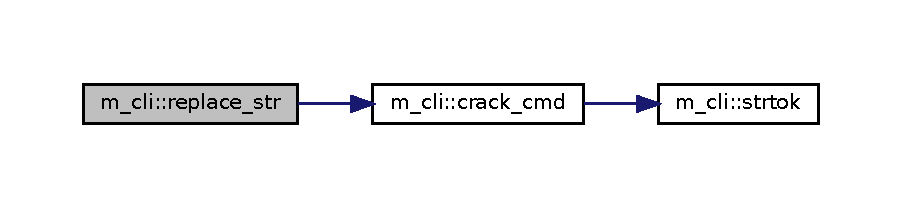
\includegraphics[width=350pt]{namespacem__cli_a40e02b1c9fc580ddd410bb24017fab8c_cgraph}
\end{center}
\end{figure}
Here is the caller graph for this function\+:\nopagebreak
\begin{figure}[H]
\begin{center}
\leavevmode
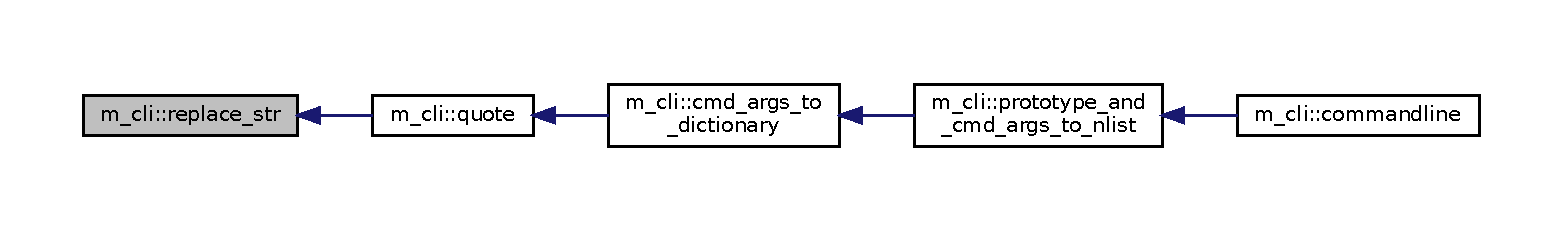
\includegraphics[width=350pt]{namespacem__cli_a40e02b1c9fc580ddd410bb24017fab8c_icgraph}
\end{center}
\end{figure}
\mbox{\Hypertarget{namespacem__cli_a0015c38f9fa45a58ba6ae89f2ddb54f1}\label{namespacem__cli_a0015c38f9fa45a58ba6ae89f2ddb54f1}} 
\index{m\+\_\+cli@{m\+\_\+cli}!strtok@{strtok}}
\index{strtok@{strtok}!m\+\_\+cli@{m\+\_\+cli}}
\subsubsection{\texorpdfstring{strtok()}{strtok()}}
{\footnotesize\ttfamily logical function m\+\_\+cli\+::strtok (\begin{DoxyParamCaption}\item[{character(len=$\ast$), intent(in)}]{source\+\_\+string,  }\item[{integer, intent(inout)}]{itoken,  }\item[{integer, intent(out)}]{token\+\_\+start,  }\item[{integer, intent(inout)}]{token\+\_\+end,  }\item[{character(len=$\ast$), intent(in)}]{delimiters }\end{DoxyParamCaption})\hspace{0.3cm}{\ttfamily [private]}}

Here is the caller graph for this function\+:\nopagebreak
\begin{figure}[H]
\begin{center}
\leavevmode
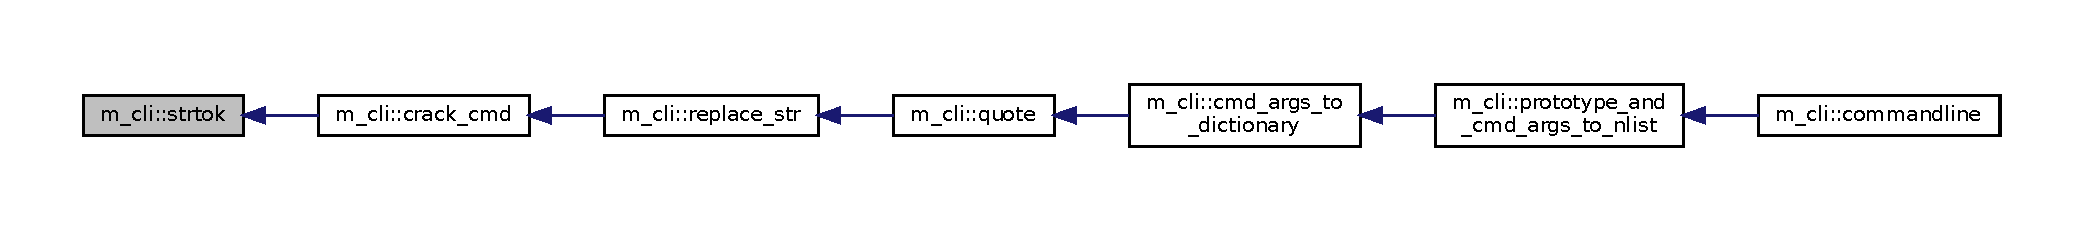
\includegraphics[width=350pt]{namespacem__cli_a0015c38f9fa45a58ba6ae89f2ddb54f1_icgraph}
\end{center}
\end{figure}
\mbox{\Hypertarget{namespacem__cli_a3b66fe9cee0e084068051636afb2957d}\label{namespacem__cli_a3b66fe9cee0e084068051636afb2957d}} 
\index{m\+\_\+cli@{m\+\_\+cli}!substitute@{substitute}}
\index{substitute@{substitute}!m\+\_\+cli@{m\+\_\+cli}}
\subsubsection{\texorpdfstring{substitute()}{substitute()}}
{\footnotesize\ttfamily subroutine m\+\_\+cli\+::substitute (\begin{DoxyParamCaption}\item[{character(len=$\ast$)}]{targetline,  }\item[{character(len=$\ast$), intent(in)}]{old,  }\item[{character(len=$\ast$), intent(in)}]{new,  }\item[{integer, intent(out), optional}]{ierr,  }\item[{integer, intent(in), optional}]{start,  }\item[{integer, intent(in), optional}]{end }\end{DoxyParamCaption})\hspace{0.3cm}{\ttfamily [private]}}

Here is the caller graph for this function\+:\nopagebreak
\begin{figure}[H]
\begin{center}
\leavevmode
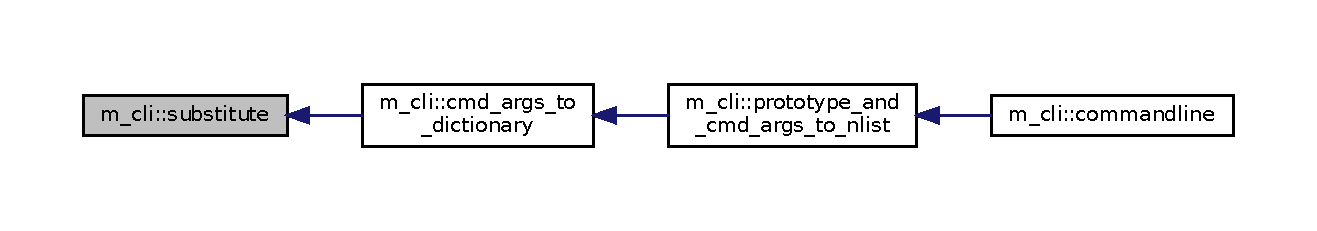
\includegraphics[width=350pt]{namespacem__cli_a3b66fe9cee0e084068051636afb2957d_icgraph}
\end{center}
\end{figure}
\mbox{\Hypertarget{namespacem__cli_a9b7676d796e5cb878ecd9294b8a689cb}\label{namespacem__cli_a9b7676d796e5cb878ecd9294b8a689cb}} 
\index{m\+\_\+cli@{m\+\_\+cli}!update@{update}}
\index{update@{update}!m\+\_\+cli@{m\+\_\+cli}}
\subsubsection{\texorpdfstring{update()}{update()}}
{\footnotesize\ttfamily subroutine, private m\+\_\+cli\+::update (\begin{DoxyParamCaption}\item[{character(len=$\ast$), intent(in)}]{key,  }\item[{character(len=$\ast$), intent(in), optional}]{val }\end{DoxyParamCaption})\hspace{0.3cm}{\ttfamily [private]}}



References counts, debug, keywords, present\+\_\+in, and values.

Here is the caller graph for this function\+:\nopagebreak
\begin{figure}[H]
\begin{center}
\leavevmode
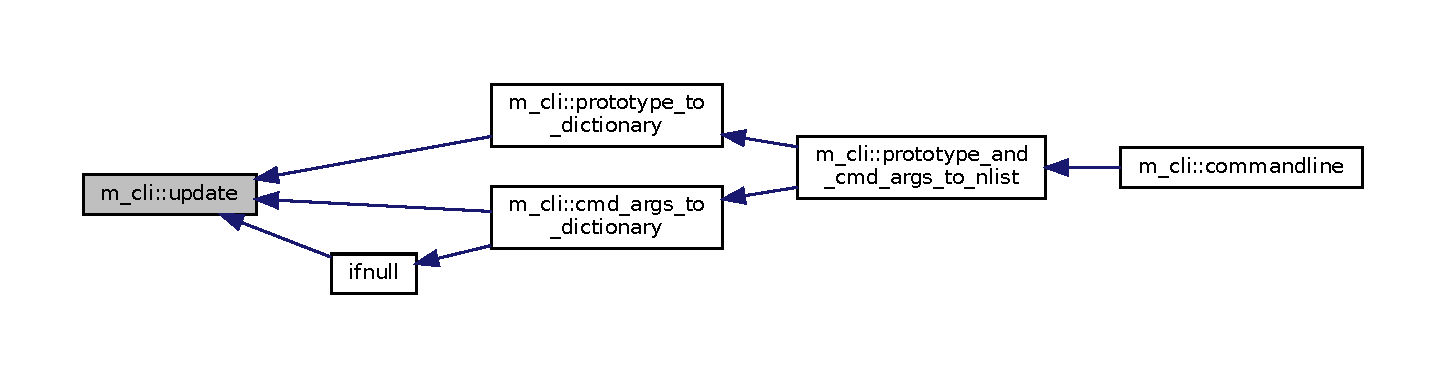
\includegraphics[width=350pt]{namespacem__cli_a9b7676d796e5cb878ecd9294b8a689cb_icgraph}
\end{center}
\end{figure}
\mbox{\Hypertarget{namespacem__cli_aef6f54c9cb37251dfd664c0845186a40}\label{namespacem__cli_aef6f54c9cb37251dfd664c0845186a40}} 
\index{m\+\_\+cli@{m\+\_\+cli}!upper@{upper}}
\index{upper@{upper}!m\+\_\+cli@{m\+\_\+cli}}
\subsubsection{\texorpdfstring{upper()}{upper()}}
{\footnotesize\ttfamily elemental pure character(len(str)) function m\+\_\+cli\+::upper (\begin{DoxyParamCaption}\item[{character($\ast$), intent(in)}]{str,  }\item[{integer, intent(in), optional}]{begin,  }\item[{integer, intent(in), optional}]{end }\end{DoxyParamCaption})\hspace{0.3cm}{\ttfamily [private]}}

Here is the caller graph for this function\+:\nopagebreak
\begin{figure}[H]
\begin{center}
\leavevmode
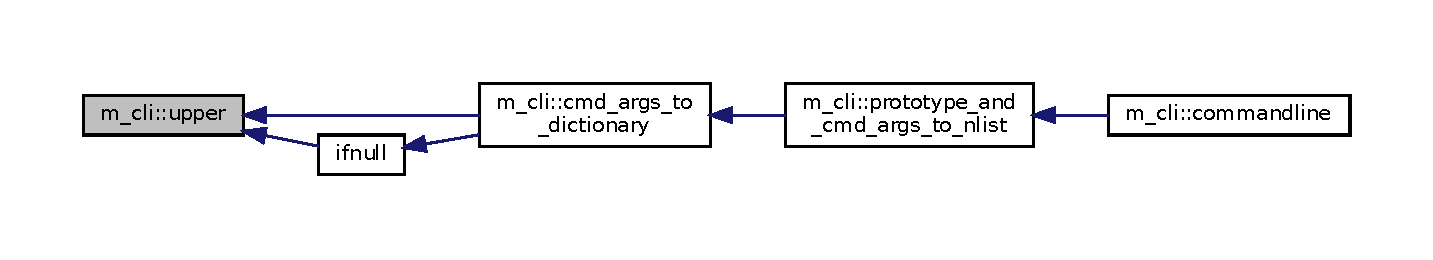
\includegraphics[width=350pt]{namespacem__cli_aef6f54c9cb37251dfd664c0845186a40_icgraph}
\end{center}
\end{figure}
\mbox{\Hypertarget{namespacem__cli_a3c1b30406fc692841826be979726bb1b}\label{namespacem__cli_a3c1b30406fc692841826be979726bb1b}} 
\index{m\+\_\+cli@{m\+\_\+cli}!wipe\+\_\+dictionary@{wipe\+\_\+dictionary}}
\index{wipe\+\_\+dictionary@{wipe\+\_\+dictionary}!m\+\_\+cli@{m\+\_\+cli}}
\subsubsection{\texorpdfstring{wipe\+\_\+dictionary()}{wipe\_dictionary()}}
{\footnotesize\ttfamily subroutine, private m\+\_\+cli\+::wipe\+\_\+dictionary (\begin{DoxyParamCaption}{ }\end{DoxyParamCaption})\hspace{0.3cm}{\ttfamily [private]}}



References counts, keywords, present\+\_\+in, and values.

Here is the caller graph for this function\+:\nopagebreak
\begin{figure}[H]
\begin{center}
\leavevmode
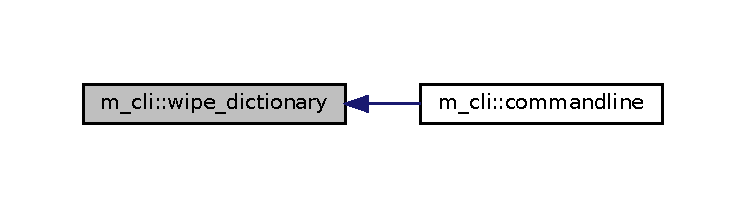
\includegraphics[width=350pt]{namespacem__cli_a3c1b30406fc692841826be979726bb1b_icgraph}
\end{center}
\end{figure}


\subsection{Variable Documentation}
\mbox{\Hypertarget{namespacem__cli_ac6af3775222feedc5aff5874ce63897a}\label{namespacem__cli_ac6af3775222feedc5aff5874ce63897a}} 
\index{m\+\_\+cli@{m\+\_\+cli}!counts@{counts}}
\index{counts@{counts}!m\+\_\+cli@{m\+\_\+cli}}
\subsubsection{\texorpdfstring{counts}{counts}}
{\footnotesize\ttfamily integer, dimension(\+:), allocatable m\+\_\+cli\+::counts\hspace{0.3cm}{\ttfamily [private]}}

\mbox{\Hypertarget{namespacem__cli_a83b45c240c1c7309a38c358ebcde28ec}\label{namespacem__cli_a83b45c240c1c7309a38c358ebcde28ec}} 
\index{m\+\_\+cli@{m\+\_\+cli}!debug@{debug}}
\index{debug@{debug}!m\+\_\+cli@{m\+\_\+cli}}
\subsubsection{\texorpdfstring{debug}{debug}}
{\footnotesize\ttfamily logical, public m\+\_\+cli\+::debug =.false.}

\mbox{\Hypertarget{namespacem__cli_acd2598fd229b4b584315292251217c31}\label{namespacem__cli_acd2598fd229b4b584315292251217c31}} 
\index{m\+\_\+cli@{m\+\_\+cli}!g\+\_\+namelist\+\_\+name@{g\+\_\+namelist\+\_\+name}}
\index{g\+\_\+namelist\+\_\+name@{g\+\_\+namelist\+\_\+name}!m\+\_\+cli@{m\+\_\+cli}}
\subsubsection{\texorpdfstring{g\+\_\+namelist\+\_\+name}{g\_namelist\_name}}
{\footnotesize\ttfamily character(len=\+:), allocatable m\+\_\+cli\+::g\+\_\+namelist\+\_\+name\hspace{0.3cm}{\ttfamily [private]}}

\mbox{\Hypertarget{namespacem__cli_a456bb87244997f19111533666a96b9eb}\label{namespacem__cli_a456bb87244997f19111533666a96b9eb}} 
\index{m\+\_\+cli@{m\+\_\+cli}!g\+\_\+noquote@{g\+\_\+noquote}}
\index{g\+\_\+noquote@{g\+\_\+noquote}!m\+\_\+cli@{m\+\_\+cli}}
\subsubsection{\texorpdfstring{g\+\_\+noquote}{g\_noquote}}
{\footnotesize\ttfamily logical m\+\_\+cli\+::g\+\_\+noquote\hspace{0.3cm}{\ttfamily [private]}}

\mbox{\Hypertarget{namespacem__cli_a179ac9786afe3fe8474d97ac1a4f1d4c}\label{namespacem__cli_a179ac9786afe3fe8474d97ac1a4f1d4c}} 
\index{m\+\_\+cli@{m\+\_\+cli}!keyword\+\_\+single@{keyword\+\_\+single}}
\index{keyword\+\_\+single@{keyword\+\_\+single}!m\+\_\+cli@{m\+\_\+cli}}
\subsubsection{\texorpdfstring{keyword\+\_\+single}{keyword\_single}}
{\footnotesize\ttfamily logical m\+\_\+cli\+::keyword\+\_\+single =.true.\hspace{0.3cm}{\ttfamily [private]}}

\mbox{\Hypertarget{namespacem__cli_a1eb7801692b3d6e25f16885fdf027f42}\label{namespacem__cli_a1eb7801692b3d6e25f16885fdf027f42}} 
\index{m\+\_\+cli@{m\+\_\+cli}!keywords@{keywords}}
\index{keywords@{keywords}!m\+\_\+cli@{m\+\_\+cli}}
\subsubsection{\texorpdfstring{keywords}{keywords}}
{\footnotesize\ttfamily character(len=\+:), dimension(\+:), allocatable m\+\_\+cli\+::keywords\hspace{0.3cm}{\ttfamily [private]}}

\mbox{\Hypertarget{namespacem__cli_aedc9f3e906ef523605292fd8cf8b00c0}\label{namespacem__cli_aedc9f3e906ef523605292fd8cf8b00c0}} 
\index{m\+\_\+cli@{m\+\_\+cli}!passed\+\_\+in@{passed\+\_\+in}}
\index{passed\+\_\+in@{passed\+\_\+in}!m\+\_\+cli@{m\+\_\+cli}}
\subsubsection{\texorpdfstring{passed\+\_\+in}{passed\_in}}
{\footnotesize\ttfamily character(len=\+:), allocatable m\+\_\+cli\+::passed\+\_\+in\hspace{0.3cm}{\ttfamily [private]}}

\mbox{\Hypertarget{namespacem__cli_ad08e57d14b3543d476d00e6bfda58fa5}\label{namespacem__cli_ad08e57d14b3543d476d00e6bfda58fa5}} 
\index{m\+\_\+cli@{m\+\_\+cli}!present\+\_\+in@{present\+\_\+in}}
\index{present\+\_\+in@{present\+\_\+in}!m\+\_\+cli@{m\+\_\+cli}}
\subsubsection{\texorpdfstring{present\+\_\+in}{present\_in}}
{\footnotesize\ttfamily logical, dimension(\+:), allocatable m\+\_\+cli\+::present\+\_\+in\hspace{0.3cm}{\ttfamily [private]}}

\mbox{\Hypertarget{namespacem__cli_a0320cf9d95b01ffbbd8f5a2e0d01ff26}\label{namespacem__cli_a0320cf9d95b01ffbbd8f5a2e0d01ff26}} 
\index{m\+\_\+cli@{m\+\_\+cli}!return\+\_\+all@{return\+\_\+all}}
\index{return\+\_\+all@{return\+\_\+all}!m\+\_\+cli@{m\+\_\+cli}}
\subsubsection{\texorpdfstring{return\+\_\+all}{return\_all}}
{\footnotesize\ttfamily logical m\+\_\+cli\+::return\+\_\+all\hspace{0.3cm}{\ttfamily [private]}}

\mbox{\Hypertarget{namespacem__cli_a7fd43837c254f34109d9f523c66c873a}\label{namespacem__cli_a7fd43837c254f34109d9f523c66c873a}} 
\index{m\+\_\+cli@{m\+\_\+cli}!unnamed@{unnamed}}
\index{unnamed@{unnamed}!m\+\_\+cli@{m\+\_\+cli}}
\subsubsection{\texorpdfstring{unnamed}{unnamed}}
{\footnotesize\ttfamily character(len=\+:), dimension(\+:), allocatable, public m\+\_\+cli\+::unnamed}

\mbox{\Hypertarget{namespacem__cli_aaec25aa63c2964c1125b9f14f27bf44a}\label{namespacem__cli_aaec25aa63c2964c1125b9f14f27bf44a}} 
\index{m\+\_\+cli@{m\+\_\+cli}!values@{values}}
\index{values@{values}!m\+\_\+cli@{m\+\_\+cli}}
\subsubsection{\texorpdfstring{values}{values}}
{\footnotesize\ttfamily character(len=\+:), dimension(\+:), allocatable m\+\_\+cli\+::values\hspace{0.3cm}{\ttfamily [private]}}


\chapter{Data Type Documentation}
\hypertarget{structm__cli_1_1dictionary}{}\section{m\+\_\+cli\+:\+:dictionary Type Reference}
\label{structm__cli_1_1dictionary}\index{m\+\_\+cli\+::dictionary@{m\+\_\+cli\+::dictionary}}
\subsection*{Private Member Functions}
\begin{DoxyCompactItemize}
\item 
procedure, private \mbox{\hyperlink{structm__cli_1_1dictionary_a00a446dbb6b83b8656f681c5d8ee6c3b}{get}} =$>$ \mbox{\hyperlink{namespacem__cli_ac4a889309ffc333af6bf8e11f1fc4869}{dict\+\_\+get}}
\item 
procedure, private \mbox{\hyperlink{structm__cli_1_1dictionary_adb28601e3f877106d0dfd143b72cd8a4}{set}} =$>$ \mbox{\hyperlink{namespacem__cli_a1be098e2b920e8d50ed14be03a3133db}{dict\+\_\+add}}
\item 
procedure, private \mbox{\hyperlink{structm__cli_1_1dictionary_aea651d5f1d801e67a9af3ebb863c537c}{del}} =$>$ \mbox{\hyperlink{namespacem__cli_aff32e44070983c7fb4eb0a3b1dea7a6d}{dict\+\_\+delete}}
\end{DoxyCompactItemize}
\subsection*{Private Attributes}
\begin{DoxyCompactItemize}
\item 
character(len=\+:), dimension(\+:), allocatable \mbox{\hyperlink{structm__cli_1_1dictionary_a78ba0e921972470e53589478dd87111f}{key}}
\item 
character(len=\+:), dimension(\+:), allocatable \mbox{\hyperlink{structm__cli_1_1dictionary_ae0e73cb96f08397f3dcbba02d2549430}{value}}
\item 
integer, dimension(\+:), allocatable \mbox{\hyperlink{structm__cli_1_1dictionary_aa83a3a6f250e1ff009492ff5c7926877}{count}}
\end{DoxyCompactItemize}


\subsection{Member Function/\+Subroutine Documentation}
\mbox{\Hypertarget{structm__cli_1_1dictionary_aea651d5f1d801e67a9af3ebb863c537c}\label{structm__cli_1_1dictionary_aea651d5f1d801e67a9af3ebb863c537c}} 
\index{m\+\_\+cli\+::dictionary@{m\+\_\+cli\+::dictionary}!del@{del}}
\index{del@{del}!m\+\_\+cli\+::dictionary@{m\+\_\+cli\+::dictionary}}
\subsubsection{\texorpdfstring{del()}{del()}}
{\footnotesize\ttfamily procedure, private m\+\_\+cli\+::dictionary\+::del (\begin{DoxyParamCaption}{ }\end{DoxyParamCaption})\hspace{0.3cm}{\ttfamily [private]}}



References m\+\_\+cli\+::insert\+\_\+c(), m\+\_\+cli\+::insert\+\_\+d(), m\+\_\+cli\+::insert\+\_\+i(), m\+\_\+cli\+::insert\+\_\+l(), m\+\_\+cli\+::insert\+\_\+r(), m\+\_\+cli\+::locate\+\_\+c(), m\+\_\+cli\+::locate\+\_\+d(), m\+\_\+cli\+::locate\+\_\+i(), m\+\_\+cli\+::locate\+\_\+r(), m\+\_\+cli\+::remove\+\_\+c(), m\+\_\+cli\+::remove\+\_\+d(), m\+\_\+cli\+::remove\+\_\+i(), m\+\_\+cli\+::remove\+\_\+l(), m\+\_\+cli\+::remove\+\_\+r(), m\+\_\+cli\+::replace\+\_\+c(), m\+\_\+cli\+::replace\+\_\+d(), m\+\_\+cli\+::replace\+\_\+i(), m\+\_\+cli\+::replace\+\_\+l(), and m\+\_\+cli\+::replace\+\_\+r().

Here is the call graph for this function\+:\nopagebreak
\begin{figure}[H]
\begin{center}
\leavevmode
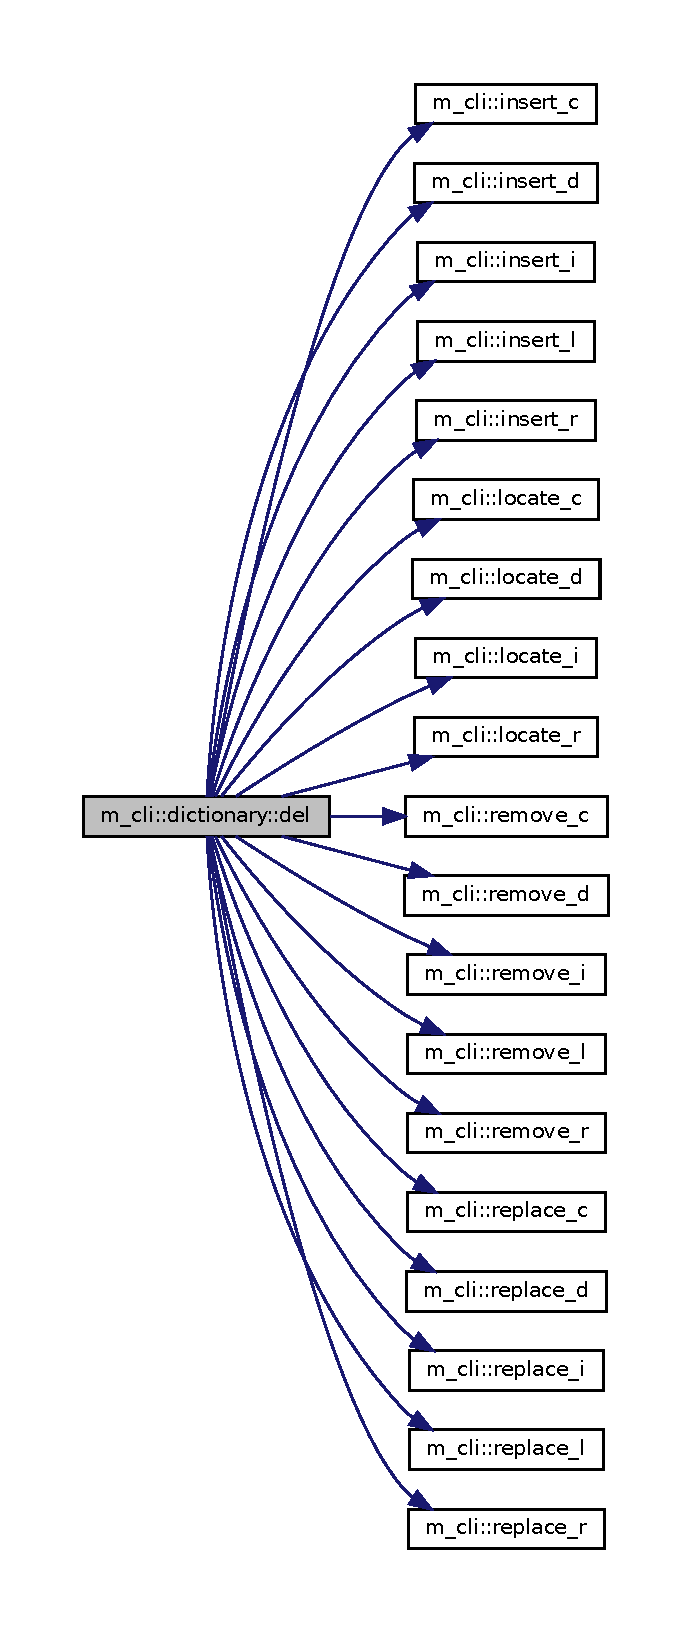
\includegraphics[height=550pt]{structm__cli_1_1dictionary_aea651d5f1d801e67a9af3ebb863c537c_cgraph}
\end{center}
\end{figure}
\mbox{\Hypertarget{structm__cli_1_1dictionary_a00a446dbb6b83b8656f681c5d8ee6c3b}\label{structm__cli_1_1dictionary_a00a446dbb6b83b8656f681c5d8ee6c3b}} 
\index{m\+\_\+cli\+::dictionary@{m\+\_\+cli\+::dictionary}!get@{get}}
\index{get@{get}!m\+\_\+cli\+::dictionary@{m\+\_\+cli\+::dictionary}}
\subsubsection{\texorpdfstring{get()}{get()}}
{\footnotesize\ttfamily procedure, private m\+\_\+cli\+::dictionary\+::get (\begin{DoxyParamCaption}{ }\end{DoxyParamCaption})\hspace{0.3cm}{\ttfamily [private]}}

\mbox{\Hypertarget{structm__cli_1_1dictionary_adb28601e3f877106d0dfd143b72cd8a4}\label{structm__cli_1_1dictionary_adb28601e3f877106d0dfd143b72cd8a4}} 
\index{m\+\_\+cli\+::dictionary@{m\+\_\+cli\+::dictionary}!set@{set}}
\index{set@{set}!m\+\_\+cli\+::dictionary@{m\+\_\+cli\+::dictionary}}
\subsubsection{\texorpdfstring{set()}{set()}}
{\footnotesize\ttfamily procedure, private m\+\_\+cli\+::dictionary\+::set (\begin{DoxyParamCaption}{ }\end{DoxyParamCaption})\hspace{0.3cm}{\ttfamily [private]}}



\subsection{Member Data Documentation}
\mbox{\Hypertarget{structm__cli_1_1dictionary_aa83a3a6f250e1ff009492ff5c7926877}\label{structm__cli_1_1dictionary_aa83a3a6f250e1ff009492ff5c7926877}} 
\index{m\+\_\+cli\+::dictionary@{m\+\_\+cli\+::dictionary}!count@{count}}
\index{count@{count}!m\+\_\+cli\+::dictionary@{m\+\_\+cli\+::dictionary}}
\subsubsection{\texorpdfstring{count}{count}}
{\footnotesize\ttfamily integer, dimension(\+:), allocatable m\+\_\+cli\+::dictionary\+::count\hspace{0.3cm}{\ttfamily [private]}}

\mbox{\Hypertarget{structm__cli_1_1dictionary_a78ba0e921972470e53589478dd87111f}\label{structm__cli_1_1dictionary_a78ba0e921972470e53589478dd87111f}} 
\index{m\+\_\+cli\+::dictionary@{m\+\_\+cli\+::dictionary}!key@{key}}
\index{key@{key}!m\+\_\+cli\+::dictionary@{m\+\_\+cli\+::dictionary}}
\subsubsection{\texorpdfstring{key}{key}}
{\footnotesize\ttfamily character(len=\+:), dimension(\+:), allocatable m\+\_\+cli\+::dictionary\+::key\hspace{0.3cm}{\ttfamily [private]}}

\mbox{\Hypertarget{structm__cli_1_1dictionary_ae0e73cb96f08397f3dcbba02d2549430}\label{structm__cli_1_1dictionary_ae0e73cb96f08397f3dcbba02d2549430}} 
\index{m\+\_\+cli\+::dictionary@{m\+\_\+cli\+::dictionary}!value@{value}}
\index{value@{value}!m\+\_\+cli\+::dictionary@{m\+\_\+cli\+::dictionary}}
\subsubsection{\texorpdfstring{value}{value}}
{\footnotesize\ttfamily character(len=\+:), dimension(\+:), allocatable m\+\_\+cli\+::dictionary\+::value\hspace{0.3cm}{\ttfamily [private]}}



The documentation for this type was generated from the following file\+:\begin{DoxyCompactItemize}
\item 
/home/urbanjs/venus/\+V600/github/\+M\+\_\+\+C\+L\+I/src/\mbox{\hyperlink{M__CLI_8f90}{M\+\_\+\+C\+L\+I.\+f90}}\end{DoxyCompactItemize}

\hypertarget{interfacem__cli_1_1insert}{}\section{m\+\_\+cli\+:\+:insert Interface Reference}
\label{interfacem__cli_1_1insert}\index{m\+\_\+cli\+::insert@{m\+\_\+cli\+::insert}}
\subsection*{Private Member Functions}
\begin{DoxyCompactItemize}
\item 
subroutine \mbox{\hyperlink{interfacem__cli_1_1insert_aca6814eaf24391cb47c31596671d8475}{insert\+\_\+c}} (list, value, place)
\item 
subroutine \mbox{\hyperlink{interfacem__cli_1_1insert_a754e4845aabebdb9c34a928f49cdaa59}{insert\+\_\+d}} (list, value, place)
\item 
subroutine \mbox{\hyperlink{interfacem__cli_1_1insert_af953a8b23ca38f6a5e123d616ad80964}{insert\+\_\+r}} (list, value, place)
\item 
subroutine \mbox{\hyperlink{interfacem__cli_1_1insert_adc369899b95770d6a3e40b22945014d0}{insert\+\_\+i}} (list, value, place)
\item 
subroutine \mbox{\hyperlink{interfacem__cli_1_1insert_a058a7eb2f5a375bd7a27cabcba64c717}{insert\+\_\+l}} (list, value, place)
\end{DoxyCompactItemize}


\subsection{Member Function/\+Subroutine Documentation}
\mbox{\Hypertarget{interfacem__cli_1_1insert_aca6814eaf24391cb47c31596671d8475}\label{interfacem__cli_1_1insert_aca6814eaf24391cb47c31596671d8475}} 
\index{m\+\_\+cli\+::insert@{m\+\_\+cli\+::insert}!insert\+\_\+c@{insert\+\_\+c}}
\index{insert\+\_\+c@{insert\+\_\+c}!m\+\_\+cli\+::insert@{m\+\_\+cli\+::insert}}
\subsubsection{\texorpdfstring{insert\+\_\+c()}{insert\_c()}}
{\footnotesize\ttfamily subroutine m\+\_\+cli\+::insert\+::insert\+\_\+c (\begin{DoxyParamCaption}\item[{character(len=\+:), dimension(\+:), allocatable}]{list,  }\item[{character(len=$\ast$), intent(in)}]{value,  }\item[{integer, intent(in)}]{place }\end{DoxyParamCaption})\hspace{0.3cm}{\ttfamily [private]}}

\mbox{\Hypertarget{interfacem__cli_1_1insert_a754e4845aabebdb9c34a928f49cdaa59}\label{interfacem__cli_1_1insert_a754e4845aabebdb9c34a928f49cdaa59}} 
\index{m\+\_\+cli\+::insert@{m\+\_\+cli\+::insert}!insert\+\_\+d@{insert\+\_\+d}}
\index{insert\+\_\+d@{insert\+\_\+d}!m\+\_\+cli\+::insert@{m\+\_\+cli\+::insert}}
\subsubsection{\texorpdfstring{insert\+\_\+d()}{insert\_d()}}
{\footnotesize\ttfamily subroutine m\+\_\+cli\+::insert\+::insert\+\_\+d (\begin{DoxyParamCaption}\item[{doubleprecision, dimension(\+:), allocatable}]{list,  }\item[{doubleprecision, intent(in)}]{value,  }\item[{integer, intent(in)}]{place }\end{DoxyParamCaption})\hspace{0.3cm}{\ttfamily [private]}}

\mbox{\Hypertarget{interfacem__cli_1_1insert_adc369899b95770d6a3e40b22945014d0}\label{interfacem__cli_1_1insert_adc369899b95770d6a3e40b22945014d0}} 
\index{m\+\_\+cli\+::insert@{m\+\_\+cli\+::insert}!insert\+\_\+i@{insert\+\_\+i}}
\index{insert\+\_\+i@{insert\+\_\+i}!m\+\_\+cli\+::insert@{m\+\_\+cli\+::insert}}
\subsubsection{\texorpdfstring{insert\+\_\+i()}{insert\_i()}}
{\footnotesize\ttfamily subroutine m\+\_\+cli\+::insert\+::insert\+\_\+i (\begin{DoxyParamCaption}\item[{integer, dimension(\+:), allocatable}]{list,  }\item[{integer, intent(in)}]{value,  }\item[{integer, intent(in)}]{place }\end{DoxyParamCaption})\hspace{0.3cm}{\ttfamily [private]}}

\mbox{\Hypertarget{interfacem__cli_1_1insert_a058a7eb2f5a375bd7a27cabcba64c717}\label{interfacem__cli_1_1insert_a058a7eb2f5a375bd7a27cabcba64c717}} 
\index{m\+\_\+cli\+::insert@{m\+\_\+cli\+::insert}!insert\+\_\+l@{insert\+\_\+l}}
\index{insert\+\_\+l@{insert\+\_\+l}!m\+\_\+cli\+::insert@{m\+\_\+cli\+::insert}}
\subsubsection{\texorpdfstring{insert\+\_\+l()}{insert\_l()}}
{\footnotesize\ttfamily subroutine m\+\_\+cli\+::insert\+::insert\+\_\+l (\begin{DoxyParamCaption}\item[{logical, dimension(\+:), allocatable}]{list,  }\item[{logical, intent(in)}]{value,  }\item[{integer, intent(in)}]{place }\end{DoxyParamCaption})\hspace{0.3cm}{\ttfamily [private]}}

\mbox{\Hypertarget{interfacem__cli_1_1insert_af953a8b23ca38f6a5e123d616ad80964}\label{interfacem__cli_1_1insert_af953a8b23ca38f6a5e123d616ad80964}} 
\index{m\+\_\+cli\+::insert@{m\+\_\+cli\+::insert}!insert\+\_\+r@{insert\+\_\+r}}
\index{insert\+\_\+r@{insert\+\_\+r}!m\+\_\+cli\+::insert@{m\+\_\+cli\+::insert}}
\subsubsection{\texorpdfstring{insert\+\_\+r()}{insert\_r()}}
{\footnotesize\ttfamily subroutine m\+\_\+cli\+::insert\+::insert\+\_\+r (\begin{DoxyParamCaption}\item[{real, dimension(\+:), allocatable}]{list,  }\item[{real, intent(in)}]{value,  }\item[{integer, intent(in)}]{place }\end{DoxyParamCaption})\hspace{0.3cm}{\ttfamily [private]}}



The documentation for this interface was generated from the following file\+:\begin{DoxyCompactItemize}
\item 
/home/urbanjs/venus/\+V600/github/\+M\+\_\+\+C\+L\+I/src/\mbox{\hyperlink{M__CLI_8f90}{M\+\_\+\+C\+L\+I.\+f90}}\end{DoxyCompactItemize}

\hypertarget{interfacem__cli_1_1locate}{}\section{m\+\_\+cli\+:\+:locate Interface Reference}
\label{interfacem__cli_1_1locate}\index{m\+\_\+cli\+::locate@{m\+\_\+cli\+::locate}}
\subsection*{Private Member Functions}
\begin{DoxyCompactItemize}
\item 
subroutine \mbox{\hyperlink{interfacem__cli_1_1locate_a785f3dd46c06df9527629c691153a30b}{locate\+\_\+c}} (list, value, place, ier, errmsg)
\item 
subroutine \mbox{\hyperlink{interfacem__cli_1_1locate_a71019028d011617570317ae09899b86a}{locate\+\_\+d}} (list, value, place, ier, errmsg)
\item 
subroutine \mbox{\hyperlink{interfacem__cli_1_1locate_a128461b6770cea9575da2b98f9803dfb}{locate\+\_\+r}} (list, value, place, ier, errmsg)
\item 
subroutine \mbox{\hyperlink{interfacem__cli_1_1locate_af977558244f03daa06eef8520a5475cc}{locate\+\_\+i}} (list, value, place, ier, errmsg)
\end{DoxyCompactItemize}


\subsection{Member Function/\+Subroutine Documentation}
\mbox{\Hypertarget{interfacem__cli_1_1locate_a785f3dd46c06df9527629c691153a30b}\label{interfacem__cli_1_1locate_a785f3dd46c06df9527629c691153a30b}} 
\index{m\+\_\+cli\+::locate@{m\+\_\+cli\+::locate}!locate\+\_\+c@{locate\+\_\+c}}
\index{locate\+\_\+c@{locate\+\_\+c}!m\+\_\+cli\+::locate@{m\+\_\+cli\+::locate}}
\subsubsection{\texorpdfstring{locate\+\_\+c()}{locate\_c()}}
{\footnotesize\ttfamily subroutine m\+\_\+cli\+::locate\+::locate\+\_\+c (\begin{DoxyParamCaption}\item[{character(len=\+:), dimension(\+:), allocatable}]{list,  }\item[{character(len=$\ast$), intent(in)}]{value,  }\item[{integer, intent(out)}]{place,  }\item[{integer, intent(out), optional}]{ier,  }\item[{character(len=$\ast$), intent(out), optional}]{errmsg }\end{DoxyParamCaption})\hspace{0.3cm}{\ttfamily [private]}}

\mbox{\Hypertarget{interfacem__cli_1_1locate_a71019028d011617570317ae09899b86a}\label{interfacem__cli_1_1locate_a71019028d011617570317ae09899b86a}} 
\index{m\+\_\+cli\+::locate@{m\+\_\+cli\+::locate}!locate\+\_\+d@{locate\+\_\+d}}
\index{locate\+\_\+d@{locate\+\_\+d}!m\+\_\+cli\+::locate@{m\+\_\+cli\+::locate}}
\subsubsection{\texorpdfstring{locate\+\_\+d()}{locate\_d()}}
{\footnotesize\ttfamily subroutine m\+\_\+cli\+::locate\+::locate\+\_\+d (\begin{DoxyParamCaption}\item[{doubleprecision, dimension(\+:), allocatable}]{list,  }\item[{doubleprecision, intent(in)}]{value,  }\item[{integer, intent(out)}]{place,  }\item[{integer, intent(out), optional}]{ier,  }\item[{character(len=$\ast$), intent(out), optional}]{errmsg }\end{DoxyParamCaption})\hspace{0.3cm}{\ttfamily [private]}}

\mbox{\Hypertarget{interfacem__cli_1_1locate_af977558244f03daa06eef8520a5475cc}\label{interfacem__cli_1_1locate_af977558244f03daa06eef8520a5475cc}} 
\index{m\+\_\+cli\+::locate@{m\+\_\+cli\+::locate}!locate\+\_\+i@{locate\+\_\+i}}
\index{locate\+\_\+i@{locate\+\_\+i}!m\+\_\+cli\+::locate@{m\+\_\+cli\+::locate}}
\subsubsection{\texorpdfstring{locate\+\_\+i()}{locate\_i()}}
{\footnotesize\ttfamily subroutine m\+\_\+cli\+::locate\+::locate\+\_\+i (\begin{DoxyParamCaption}\item[{integer, dimension(\+:), allocatable}]{list,  }\item[{integer, intent(in)}]{value,  }\item[{integer, intent(out)}]{place,  }\item[{integer, intent(out), optional}]{ier,  }\item[{character(len=$\ast$), intent(out), optional}]{errmsg }\end{DoxyParamCaption})\hspace{0.3cm}{\ttfamily [private]}}

\mbox{\Hypertarget{interfacem__cli_1_1locate_a128461b6770cea9575da2b98f9803dfb}\label{interfacem__cli_1_1locate_a128461b6770cea9575da2b98f9803dfb}} 
\index{m\+\_\+cli\+::locate@{m\+\_\+cli\+::locate}!locate\+\_\+r@{locate\+\_\+r}}
\index{locate\+\_\+r@{locate\+\_\+r}!m\+\_\+cli\+::locate@{m\+\_\+cli\+::locate}}
\subsubsection{\texorpdfstring{locate\+\_\+r()}{locate\_r()}}
{\footnotesize\ttfamily subroutine m\+\_\+cli\+::locate\+::locate\+\_\+r (\begin{DoxyParamCaption}\item[{real, dimension(\+:), allocatable}]{list,  }\item[{real, intent(in)}]{value,  }\item[{integer, intent(out)}]{place,  }\item[{integer, intent(out), optional}]{ier,  }\item[{character(len=$\ast$), intent(out), optional}]{errmsg }\end{DoxyParamCaption})\hspace{0.3cm}{\ttfamily [private]}}



The documentation for this interface was generated from the following file\+:\begin{DoxyCompactItemize}
\item 
/home/urbanjs/venus/\+V600/github/\+M\+\_\+\+C\+L\+I/src/\mbox{\hyperlink{M__CLI_8f90}{M\+\_\+\+C\+L\+I.\+f90}}\end{DoxyCompactItemize}

\hypertarget{structm__cli_1_1option}{}\section{m\+\_\+cli\+:\+:option Type Reference}
\label{structm__cli_1_1option}\index{m\+\_\+cli\+::option@{m\+\_\+cli\+::option}}
\subsection*{Private Attributes}
\begin{DoxyCompactItemize}
\item 
character(\+:), allocatable \mbox{\hyperlink{structm__cli_1_1option_aa692838478185b97d4cfd1466f50bbd2}{shortname}}
\item 
character(\+:), allocatable \mbox{\hyperlink{structm__cli_1_1option_a62395dcd3084458b35eb3d17d83629e3}{longname}}
\item 
character(\+:), allocatable \mbox{\hyperlink{structm__cli_1_1option_af205e1577880efcf61a60b96b27adfcb}{value}}
\item 
integer \mbox{\hyperlink{structm__cli_1_1option_a509fac088013b99dd798fdc65ff19bd2}{length}}
\item 
logical \mbox{\hyperlink{structm__cli_1_1option_a03434888018f675f2680f5defdc4b739}{present\+\_\+in}}
\end{DoxyCompactItemize}


\subsection{Member Data Documentation}
\mbox{\Hypertarget{structm__cli_1_1option_a509fac088013b99dd798fdc65ff19bd2}\label{structm__cli_1_1option_a509fac088013b99dd798fdc65ff19bd2}} 
\index{m\+\_\+cli\+::option@{m\+\_\+cli\+::option}!length@{length}}
\index{length@{length}!m\+\_\+cli\+::option@{m\+\_\+cli\+::option}}
\subsubsection{\texorpdfstring{length}{length}}
{\footnotesize\ttfamily integer m\+\_\+cli\+::option\+::length\hspace{0.3cm}{\ttfamily [private]}}

\mbox{\Hypertarget{structm__cli_1_1option_a62395dcd3084458b35eb3d17d83629e3}\label{structm__cli_1_1option_a62395dcd3084458b35eb3d17d83629e3}} 
\index{m\+\_\+cli\+::option@{m\+\_\+cli\+::option}!longname@{longname}}
\index{longname@{longname}!m\+\_\+cli\+::option@{m\+\_\+cli\+::option}}
\subsubsection{\texorpdfstring{longname}{longname}}
{\footnotesize\ttfamily character(\+:), allocatable m\+\_\+cli\+::option\+::longname\hspace{0.3cm}{\ttfamily [private]}}

\mbox{\Hypertarget{structm__cli_1_1option_a03434888018f675f2680f5defdc4b739}\label{structm__cli_1_1option_a03434888018f675f2680f5defdc4b739}} 
\index{m\+\_\+cli\+::option@{m\+\_\+cli\+::option}!present\+\_\+in@{present\+\_\+in}}
\index{present\+\_\+in@{present\+\_\+in}!m\+\_\+cli\+::option@{m\+\_\+cli\+::option}}
\subsubsection{\texorpdfstring{present\+\_\+in}{present\_in}}
{\footnotesize\ttfamily logical m\+\_\+cli\+::option\+::present\+\_\+in\hspace{0.3cm}{\ttfamily [private]}}

\mbox{\Hypertarget{structm__cli_1_1option_aa692838478185b97d4cfd1466f50bbd2}\label{structm__cli_1_1option_aa692838478185b97d4cfd1466f50bbd2}} 
\index{m\+\_\+cli\+::option@{m\+\_\+cli\+::option}!shortname@{shortname}}
\index{shortname@{shortname}!m\+\_\+cli\+::option@{m\+\_\+cli\+::option}}
\subsubsection{\texorpdfstring{shortname}{shortname}}
{\footnotesize\ttfamily character(\+:), allocatable m\+\_\+cli\+::option\+::shortname\hspace{0.3cm}{\ttfamily [private]}}

\mbox{\Hypertarget{structm__cli_1_1option_af205e1577880efcf61a60b96b27adfcb}\label{structm__cli_1_1option_af205e1577880efcf61a60b96b27adfcb}} 
\index{m\+\_\+cli\+::option@{m\+\_\+cli\+::option}!value@{value}}
\index{value@{value}!m\+\_\+cli\+::option@{m\+\_\+cli\+::option}}
\subsubsection{\texorpdfstring{value}{value}}
{\footnotesize\ttfamily character(\+:), allocatable m\+\_\+cli\+::option\+::value\hspace{0.3cm}{\ttfamily [private]}}



The documentation for this type was generated from the following file\+:\begin{DoxyCompactItemize}
\item 
/home/urbanjs/venus/\+V600/github/\+M\+\_\+\+C\+L\+I/src/\mbox{\hyperlink{M__CLI_8f90}{M\+\_\+\+C\+L\+I.\+f90}}\end{DoxyCompactItemize}

\hypertarget{interfacem__cli_1_1remove}{}\section{m\+\_\+cli\+:\+:remove Interface Reference}
\label{interfacem__cli_1_1remove}\index{m\+\_\+cli\+::remove@{m\+\_\+cli\+::remove}}
\subsection*{Private Member Functions}
\begin{DoxyCompactItemize}
\item 
subroutine \mbox{\hyperlink{interfacem__cli_1_1remove_a3742d63ad5d2a2e916a75bae43c4422b}{remove\+\_\+c}} (list, place)
\item 
subroutine \mbox{\hyperlink{interfacem__cli_1_1remove_ab1f0d48faa67f5ada3b7c67b6c4e6efe}{remove\+\_\+d}} (list, place)
\item 
subroutine \mbox{\hyperlink{interfacem__cli_1_1remove_a37084cd7166efe0231e50a8ba9d99bac}{remove\+\_\+r}} (list, place)
\item 
subroutine \mbox{\hyperlink{interfacem__cli_1_1remove_ada40f4218cbbff786409693c0e5b4e8f}{remove\+\_\+i}} (list, place)
\item 
subroutine \mbox{\hyperlink{interfacem__cli_1_1remove_a934593716f18cbe5c58e2b0af7ddb38f}{remove\+\_\+l}} (list, place)
\end{DoxyCompactItemize}


\subsection{Member Function/\+Subroutine Documentation}
\mbox{\Hypertarget{interfacem__cli_1_1remove_a3742d63ad5d2a2e916a75bae43c4422b}\label{interfacem__cli_1_1remove_a3742d63ad5d2a2e916a75bae43c4422b}} 
\index{m\+\_\+cli\+::remove@{m\+\_\+cli\+::remove}!remove\+\_\+c@{remove\+\_\+c}}
\index{remove\+\_\+c@{remove\+\_\+c}!m\+\_\+cli\+::remove@{m\+\_\+cli\+::remove}}
\subsubsection{\texorpdfstring{remove\+\_\+c()}{remove\_c()}}
{\footnotesize\ttfamily subroutine m\+\_\+cli\+::remove\+::remove\+\_\+c (\begin{DoxyParamCaption}\item[{character(len=\+:), dimension(\+:), allocatable}]{list,  }\item[{integer, intent(in)}]{place }\end{DoxyParamCaption})\hspace{0.3cm}{\ttfamily [private]}}

\mbox{\Hypertarget{interfacem__cli_1_1remove_ab1f0d48faa67f5ada3b7c67b6c4e6efe}\label{interfacem__cli_1_1remove_ab1f0d48faa67f5ada3b7c67b6c4e6efe}} 
\index{m\+\_\+cli\+::remove@{m\+\_\+cli\+::remove}!remove\+\_\+d@{remove\+\_\+d}}
\index{remove\+\_\+d@{remove\+\_\+d}!m\+\_\+cli\+::remove@{m\+\_\+cli\+::remove}}
\subsubsection{\texorpdfstring{remove\+\_\+d()}{remove\_d()}}
{\footnotesize\ttfamily subroutine m\+\_\+cli\+::remove\+::remove\+\_\+d (\begin{DoxyParamCaption}\item[{doubleprecision, dimension(\+:), allocatable}]{list,  }\item[{integer, intent(in)}]{place }\end{DoxyParamCaption})\hspace{0.3cm}{\ttfamily [private]}}

\mbox{\Hypertarget{interfacem__cli_1_1remove_ada40f4218cbbff786409693c0e5b4e8f}\label{interfacem__cli_1_1remove_ada40f4218cbbff786409693c0e5b4e8f}} 
\index{m\+\_\+cli\+::remove@{m\+\_\+cli\+::remove}!remove\+\_\+i@{remove\+\_\+i}}
\index{remove\+\_\+i@{remove\+\_\+i}!m\+\_\+cli\+::remove@{m\+\_\+cli\+::remove}}
\subsubsection{\texorpdfstring{remove\+\_\+i()}{remove\_i()}}
{\footnotesize\ttfamily subroutine m\+\_\+cli\+::remove\+::remove\+\_\+i (\begin{DoxyParamCaption}\item[{integer, dimension(\+:), allocatable}]{list,  }\item[{integer, intent(in)}]{place }\end{DoxyParamCaption})\hspace{0.3cm}{\ttfamily [private]}}

\mbox{\Hypertarget{interfacem__cli_1_1remove_a934593716f18cbe5c58e2b0af7ddb38f}\label{interfacem__cli_1_1remove_a934593716f18cbe5c58e2b0af7ddb38f}} 
\index{m\+\_\+cli\+::remove@{m\+\_\+cli\+::remove}!remove\+\_\+l@{remove\+\_\+l}}
\index{remove\+\_\+l@{remove\+\_\+l}!m\+\_\+cli\+::remove@{m\+\_\+cli\+::remove}}
\subsubsection{\texorpdfstring{remove\+\_\+l()}{remove\_l()}}
{\footnotesize\ttfamily subroutine m\+\_\+cli\+::remove\+::remove\+\_\+l (\begin{DoxyParamCaption}\item[{logical, dimension(\+:), allocatable}]{list,  }\item[{integer, intent(in)}]{place }\end{DoxyParamCaption})\hspace{0.3cm}{\ttfamily [private]}}

\mbox{\Hypertarget{interfacem__cli_1_1remove_a37084cd7166efe0231e50a8ba9d99bac}\label{interfacem__cli_1_1remove_a37084cd7166efe0231e50a8ba9d99bac}} 
\index{m\+\_\+cli\+::remove@{m\+\_\+cli\+::remove}!remove\+\_\+r@{remove\+\_\+r}}
\index{remove\+\_\+r@{remove\+\_\+r}!m\+\_\+cli\+::remove@{m\+\_\+cli\+::remove}}
\subsubsection{\texorpdfstring{remove\+\_\+r()}{remove\_r()}}
{\footnotesize\ttfamily subroutine m\+\_\+cli\+::remove\+::remove\+\_\+r (\begin{DoxyParamCaption}\item[{real, dimension(\+:), allocatable}]{list,  }\item[{integer, intent(in)}]{place }\end{DoxyParamCaption})\hspace{0.3cm}{\ttfamily [private]}}



The documentation for this interface was generated from the following file\+:\begin{DoxyCompactItemize}
\item 
/home/urbanjs/venus/\+V600/github/\+M\+\_\+\+C\+L\+I/src/\mbox{\hyperlink{M__CLI_8f90}{M\+\_\+\+C\+L\+I.\+f90}}\end{DoxyCompactItemize}

\hypertarget{interfacem__cli_1_1replace}{}\section{m\+\_\+cli\+:\+:replace Interface Reference}
\label{interfacem__cli_1_1replace}\index{m\+\_\+cli\+::replace@{m\+\_\+cli\+::replace}}
\subsection*{Private Member Functions}
\begin{DoxyCompactItemize}
\item 
subroutine \mbox{\hyperlink{interfacem__cli_1_1replace_ae1cfecec71387e484a12f7e02416327b}{replace\+\_\+c}} (list, value, place)
\item 
subroutine \mbox{\hyperlink{interfacem__cli_1_1replace_acc8e55b73266f8ec6841359b46c032a5}{replace\+\_\+d}} (list, value, place)
\item 
subroutine \mbox{\hyperlink{interfacem__cli_1_1replace_abf109545f37e44c1f6cc0176c75ef738}{replace\+\_\+r}} (list, value, place)
\item 
subroutine \mbox{\hyperlink{interfacem__cli_1_1replace_abc84f285072aca38fb5b9464b9ee7401}{replace\+\_\+i}} (list, value, place)
\item 
subroutine \mbox{\hyperlink{interfacem__cli_1_1replace_ac9f0196d45313ed60d0c0368fc2fd444}{replace\+\_\+l}} (list, value, place)
\end{DoxyCompactItemize}


\subsection{Member Function/\+Subroutine Documentation}
\mbox{\Hypertarget{interfacem__cli_1_1replace_ae1cfecec71387e484a12f7e02416327b}\label{interfacem__cli_1_1replace_ae1cfecec71387e484a12f7e02416327b}} 
\index{m\+\_\+cli\+::replace@{m\+\_\+cli\+::replace}!replace\+\_\+c@{replace\+\_\+c}}
\index{replace\+\_\+c@{replace\+\_\+c}!m\+\_\+cli\+::replace@{m\+\_\+cli\+::replace}}
\subsubsection{\texorpdfstring{replace\+\_\+c()}{replace\_c()}}
{\footnotesize\ttfamily subroutine m\+\_\+cli\+::replace\+::replace\+\_\+c (\begin{DoxyParamCaption}\item[{character(len=\+:), dimension(\+:), allocatable}]{list,  }\item[{character(len=$\ast$), intent(in)}]{value,  }\item[{integer, intent(in)}]{place }\end{DoxyParamCaption})\hspace{0.3cm}{\ttfamily [private]}}

\mbox{\Hypertarget{interfacem__cli_1_1replace_acc8e55b73266f8ec6841359b46c032a5}\label{interfacem__cli_1_1replace_acc8e55b73266f8ec6841359b46c032a5}} 
\index{m\+\_\+cli\+::replace@{m\+\_\+cli\+::replace}!replace\+\_\+d@{replace\+\_\+d}}
\index{replace\+\_\+d@{replace\+\_\+d}!m\+\_\+cli\+::replace@{m\+\_\+cli\+::replace}}
\subsubsection{\texorpdfstring{replace\+\_\+d()}{replace\_d()}}
{\footnotesize\ttfamily subroutine m\+\_\+cli\+::replace\+::replace\+\_\+d (\begin{DoxyParamCaption}\item[{doubleprecision, dimension(\+:), allocatable}]{list,  }\item[{doubleprecision, intent(in)}]{value,  }\item[{integer, intent(in)}]{place }\end{DoxyParamCaption})\hspace{0.3cm}{\ttfamily [private]}}

\mbox{\Hypertarget{interfacem__cli_1_1replace_abc84f285072aca38fb5b9464b9ee7401}\label{interfacem__cli_1_1replace_abc84f285072aca38fb5b9464b9ee7401}} 
\index{m\+\_\+cli\+::replace@{m\+\_\+cli\+::replace}!replace\+\_\+i@{replace\+\_\+i}}
\index{replace\+\_\+i@{replace\+\_\+i}!m\+\_\+cli\+::replace@{m\+\_\+cli\+::replace}}
\subsubsection{\texorpdfstring{replace\+\_\+i()}{replace\_i()}}
{\footnotesize\ttfamily subroutine m\+\_\+cli\+::replace\+::replace\+\_\+i (\begin{DoxyParamCaption}\item[{integer, dimension(\+:), allocatable}]{list,  }\item[{integer, intent(in)}]{value,  }\item[{integer, intent(in)}]{place }\end{DoxyParamCaption})\hspace{0.3cm}{\ttfamily [private]}}

\mbox{\Hypertarget{interfacem__cli_1_1replace_ac9f0196d45313ed60d0c0368fc2fd444}\label{interfacem__cli_1_1replace_ac9f0196d45313ed60d0c0368fc2fd444}} 
\index{m\+\_\+cli\+::replace@{m\+\_\+cli\+::replace}!replace\+\_\+l@{replace\+\_\+l}}
\index{replace\+\_\+l@{replace\+\_\+l}!m\+\_\+cli\+::replace@{m\+\_\+cli\+::replace}}
\subsubsection{\texorpdfstring{replace\+\_\+l()}{replace\_l()}}
{\footnotesize\ttfamily subroutine m\+\_\+cli\+::replace\+::replace\+\_\+l (\begin{DoxyParamCaption}\item[{logical, dimension(\+:), allocatable}]{list,  }\item[{logical, intent(in)}]{value,  }\item[{integer, intent(in)}]{place }\end{DoxyParamCaption})\hspace{0.3cm}{\ttfamily [private]}}

\mbox{\Hypertarget{interfacem__cli_1_1replace_abf109545f37e44c1f6cc0176c75ef738}\label{interfacem__cli_1_1replace_abf109545f37e44c1f6cc0176c75ef738}} 
\index{m\+\_\+cli\+::replace@{m\+\_\+cli\+::replace}!replace\+\_\+r@{replace\+\_\+r}}
\index{replace\+\_\+r@{replace\+\_\+r}!m\+\_\+cli\+::replace@{m\+\_\+cli\+::replace}}
\subsubsection{\texorpdfstring{replace\+\_\+r()}{replace\_r()}}
{\footnotesize\ttfamily subroutine m\+\_\+cli\+::replace\+::replace\+\_\+r (\begin{DoxyParamCaption}\item[{real, dimension(\+:), allocatable}]{list,  }\item[{real, intent(in)}]{value,  }\item[{integer, intent(in)}]{place }\end{DoxyParamCaption})\hspace{0.3cm}{\ttfamily [private]}}



The documentation for this interface was generated from the following file\+:\begin{DoxyCompactItemize}
\item 
/home/urbanjs/venus/\+V600/github/\+M\+\_\+\+C\+L\+I/src/\mbox{\hyperlink{M__CLI_8f90}{M\+\_\+\+C\+L\+I.\+f90}}\end{DoxyCompactItemize}

\chapter{File Documentation}
\hypertarget{M__CLI_8f90}{}\section{/home/urbanjs/venus/\+V600/github/\+M\+\_\+\+C\+L\+I/src/\+M\+\_\+\+C\+LI.f90 File Reference}
\label{M__CLI_8f90}\index{/home/urbanjs/venus/\+V600/github/\+M\+\_\+\+C\+L\+I/src/\+M\+\_\+\+C\+L\+I.\+f90@{/home/urbanjs/venus/\+V600/github/\+M\+\_\+\+C\+L\+I/src/\+M\+\_\+\+C\+L\+I.\+f90}}
\subsection*{Data Types}
\begin{DoxyCompactItemize}
\item 
type \mbox{\hyperlink{structm__cli_1_1option}{m\+\_\+cli\+::option}}
\item 
type \mbox{\hyperlink{structm__cli_1_1dictionary}{m\+\_\+cli\+::dictionary}}
\item 
interface \mbox{\hyperlink{interfacem__cli_1_1locate}{m\+\_\+cli\+::locate}}
\item 
interface \mbox{\hyperlink{interfacem__cli_1_1insert}{m\+\_\+cli\+::insert}}
\item 
interface \mbox{\hyperlink{interfacem__cli_1_1replace}{m\+\_\+cli\+::replace}}
\item 
interface \mbox{\hyperlink{interfacem__cli_1_1remove}{m\+\_\+cli\+::remove}}
\end{DoxyCompactItemize}
\subsection*{Modules}
\begin{DoxyCompactItemize}
\item 
module \mbox{\hyperlink{namespacem__cli}{m\+\_\+cli}}
\end{DoxyCompactItemize}
\subsection*{Functions/\+Subroutines}
\begin{DoxyCompactItemize}
\item 
subroutine, public \mbox{\hyperlink{namespacem__cli_a62056f0c153eb63cb0b11a21edb028cd}{m\+\_\+cli\+::check\+\_\+commandline}} (ios, message, help\+\_\+text, version\+\_\+text)
\item 
character(len=\+:) function, allocatable, public \mbox{\hyperlink{namespacem__cli_a4f639b0c4bf16930fc1c5858ed4196a3}{m\+\_\+cli\+::commandline}} (definition, name, noquote)
\item 
subroutine, private \mbox{\hyperlink{namespacem__cli_a8c62537a2d224364c9cb30005be819e9}{m\+\_\+cli\+::prototype\+\_\+to\+\_\+dictionary}} (string)
\item 
subroutine, private \mbox{\hyperlink{namespacem__cli_a9b7676d796e5cb878ecd9294b8a689cb}{m\+\_\+cli\+::update}} (key, val)
\item 
subroutine, private \mbox{\hyperlink{namespacem__cli_a3c1b30406fc692841826be979726bb1b}{m\+\_\+cli\+::wipe\+\_\+dictionary}} ()
\item 
character(len=\+:) function, allocatable, private \mbox{\hyperlink{namespacem__cli_a45783c194a1484042f63c58b180ca8df}{m\+\_\+cli\+::get}} (key)
\item 
subroutine, private \mbox{\hyperlink{namespacem__cli_ac77d70573b34ade2079cc4004a6acba5}{m\+\_\+cli\+::prototype\+\_\+and\+\_\+cmd\+\_\+args\+\_\+to\+\_\+nlist}} (prototype, nml)
\item 
subroutine \mbox{\hyperlink{namespacem__cli_a89a63254465b02048f09541e51974764}{m\+\_\+cli\+::cmd\+\_\+args\+\_\+to\+\_\+dictionary}} (check)
\item 
subroutine \mbox{\hyperlink{M__CLI_8f90_aa26f90016621d1ee43d3b5b66316532b}{ifnull}} ()
\item 
subroutine \mbox{\hyperlink{namespacem__cli_a7e5041efcad56387232475a3ae728634}{m\+\_\+cli\+::dictionary\+\_\+to\+\_\+namelist}} (nml)
\item 
subroutine, public \mbox{\hyperlink{namespacem__cli_a5b6abaf1d5aec5e918be0759df29c849}{m\+\_\+cli\+::print\+\_\+dictionary}} (header, stop)
\item 
integer function, private \mbox{\hyperlink{namespacem__cli_aaf5504d3b48696a9d22fa5773c5a7d15}{m\+\_\+cli\+::longest\+\_\+command\+\_\+argument}} ()
\item 
subroutine, private \mbox{\hyperlink{namespacem__cli_ade3d1e36f0fc6a47b5469dcd8ade5312}{m\+\_\+cli\+::locate\+\_\+c}} (list, value, place, ier, errmsg)
\item 
subroutine, private \mbox{\hyperlink{namespacem__cli_a4187c24a2abf5cc630232965637493e8}{m\+\_\+cli\+::locate\+\_\+d}} (list, value, place, ier, errmsg)
\item 
subroutine, private \mbox{\hyperlink{namespacem__cli_ac44389e115b536069f324bffea7d2469}{m\+\_\+cli\+::locate\+\_\+r}} (list, value, place, ier, errmsg)
\item 
subroutine, private \mbox{\hyperlink{namespacem__cli_a36665ab0ea5080c14c8c9e52ed07d397}{m\+\_\+cli\+::locate\+\_\+i}} (list, value, place, ier, errmsg)
\item 
subroutine, private \mbox{\hyperlink{namespacem__cli_a05f549b10f50798d68003b8fd2a2d86a}{m\+\_\+cli\+::remove\+\_\+c}} (list, place)
\item 
subroutine, private \mbox{\hyperlink{namespacem__cli_abf22cbc2af66482f33b7bb1a210d9d99}{m\+\_\+cli\+::remove\+\_\+d}} (list, place)
\item 
subroutine, private \mbox{\hyperlink{namespacem__cli_a4f47701695b95c88fa4927c04996ce0f}{m\+\_\+cli\+::remove\+\_\+r}} (list, place)
\item 
subroutine, private \mbox{\hyperlink{namespacem__cli_a9c86f0f52ce71f14e774fd21f0686cf6}{m\+\_\+cli\+::remove\+\_\+l}} (list, place)
\item 
subroutine, private \mbox{\hyperlink{namespacem__cli_afa08d3d87184a6dd68a124231e536c93}{m\+\_\+cli\+::remove\+\_\+i}} (list, place)
\item 
subroutine, private \mbox{\hyperlink{namespacem__cli_a785aa0016768b6dc2e27c29d5342c329}{m\+\_\+cli\+::replace\+\_\+c}} (list, value, place)
\item 
subroutine, private \mbox{\hyperlink{namespacem__cli_aa9b7d672cc9fb0bc79fd09a2870614f5}{m\+\_\+cli\+::replace\+\_\+d}} (list, value, place)
\item 
subroutine, private \mbox{\hyperlink{namespacem__cli_ab3b33abc8a6da174d3f27c2f2203038c}{m\+\_\+cli\+::replace\+\_\+r}} (list, value, place)
\item 
subroutine, private \mbox{\hyperlink{namespacem__cli_a89ed5c3b944f91d8135173206fbc7e07}{m\+\_\+cli\+::replace\+\_\+l}} (list, value, place)
\item 
subroutine, private \mbox{\hyperlink{namespacem__cli_ac609c48bb1f904235b8cbf8bea61473f}{m\+\_\+cli\+::replace\+\_\+i}} (list, value, place)
\item 
subroutine, private \mbox{\hyperlink{namespacem__cli_a9baf1cf0e20942fbde8c025ead5a30db}{m\+\_\+cli\+::insert\+\_\+c}} (list, value, place)
\item 
subroutine, private \mbox{\hyperlink{namespacem__cli_a4bfb90e14824f94017b1d4fcb39f0701}{m\+\_\+cli\+::insert\+\_\+r}} (list, value, place)
\item 
subroutine, private \mbox{\hyperlink{namespacem__cli_a030e31579a7968aea68d80db1e36ebfd}{m\+\_\+cli\+::insert\+\_\+d}} (list, value, place)
\item 
subroutine, private \mbox{\hyperlink{namespacem__cli_a0c1b22c46470afbb4ee5c67180335578}{m\+\_\+cli\+::insert\+\_\+l}} (list, value, place)
\item 
subroutine, private \mbox{\hyperlink{namespacem__cli_a841685591ef1f1827fc1fe32a7f546f1}{m\+\_\+cli\+::insert\+\_\+i}} (list, value, place)
\item 
subroutine \mbox{\hyperlink{namespacem__cli_aff32e44070983c7fb4eb0a3b1dea7a6d}{m\+\_\+cli\+::dict\+\_\+delete}} (self, key)
\item 
character(len=\+:) function, allocatable \mbox{\hyperlink{namespacem__cli_ac4a889309ffc333af6bf8e11f1fc4869}{m\+\_\+cli\+::dict\+\_\+get}} (self, key)
\item 
subroutine \mbox{\hyperlink{namespacem__cli_a1be098e2b920e8d50ed14be03a3133db}{m\+\_\+cli\+::dict\+\_\+add}} (self, key, value)
\item 
pure elemental logical function \mbox{\hyperlink{namespacem__cli_a4c126288dc18289b2095a0882f10ca77}{m\+\_\+cli\+::isupper}} (ch)
\item 
elemental pure character(len(str)) function \mbox{\hyperlink{namespacem__cli_aef6f54c9cb37251dfd664c0845186a40}{m\+\_\+cli\+::upper}} (str, begin, end)
\item 
elemental pure character(len(str)) function \mbox{\hyperlink{namespacem__cli_a685574282a09c3f57e0c18654a3a642c}{m\+\_\+cli\+::lower}} (str, begin, end)
\item 
character(len=\+:) function, allocatable \mbox{\hyperlink{namespacem__cli_ac82fec2a5441020701fe3c64af3d9948}{m\+\_\+cli\+::quote}} (str, mode)
\item 
character(len=\+:) function, allocatable \mbox{\hyperlink{namespacem__cli_a40e02b1c9fc580ddd410bb24017fab8c}{m\+\_\+cli\+::replace\+\_\+str}} (targetline, old, new, ierr, cmd, range)
\item 
subroutine \mbox{\hyperlink{namespacem__cli_a8d5d1954aac6494e07fb11f12f635c85}{m\+\_\+cli\+::crack\+\_\+cmd}} (cmd, old, new, ierr)
\item 
logical function \mbox{\hyperlink{namespacem__cli_a0015c38f9fa45a58ba6ae89f2ddb54f1}{m\+\_\+cli\+::strtok}} (source\+\_\+string, itoken, token\+\_\+start, token\+\_\+end, delimiters)
\item 
subroutine \mbox{\hyperlink{namespacem__cli_a3b66fe9cee0e084068051636afb2957d}{m\+\_\+cli\+::substitute}} (targetline, old, new, ierr, start, end)
\end{DoxyCompactItemize}
\subsection*{Variables}
\begin{DoxyCompactItemize}
\item 
character(len=\+:), dimension(\+:), allocatable, public \mbox{\hyperlink{namespacem__cli_a7fd43837c254f34109d9f523c66c873a}{m\+\_\+cli\+::unnamed}}
\item 
character(len=\+:), dimension(\+:), allocatable \mbox{\hyperlink{namespacem__cli_a1eb7801692b3d6e25f16885fdf027f42}{m\+\_\+cli\+::keywords}}
\item 
character(len=\+:), dimension(\+:), allocatable \mbox{\hyperlink{namespacem__cli_aaec25aa63c2964c1125b9f14f27bf44a}{m\+\_\+cli\+::values}}
\item 
integer, dimension(\+:), allocatable \mbox{\hyperlink{namespacem__cli_ac6af3775222feedc5aff5874ce63897a}{m\+\_\+cli\+::counts}}
\item 
logical, dimension(\+:), allocatable \mbox{\hyperlink{namespacem__cli_ad08e57d14b3543d476d00e6bfda58fa5}{m\+\_\+cli\+::present\+\_\+in}}
\item 
logical \mbox{\hyperlink{namespacem__cli_a179ac9786afe3fe8474d97ac1a4f1d4c}{m\+\_\+cli\+::keyword\+\_\+single}} =.true.
\item 
character(len=\+:), allocatable \mbox{\hyperlink{namespacem__cli_aedc9f3e906ef523605292fd8cf8b00c0}{m\+\_\+cli\+::passed\+\_\+in}}
\item 
character(len=\+:), allocatable \mbox{\hyperlink{namespacem__cli_acd2598fd229b4b584315292251217c31}{m\+\_\+cli\+::g\+\_\+namelist\+\_\+name}}
\item 
logical \mbox{\hyperlink{namespacem__cli_a456bb87244997f19111533666a96b9eb}{m\+\_\+cli\+::g\+\_\+noquote}}
\item 
logical, public \mbox{\hyperlink{namespacem__cli_a83b45c240c1c7309a38c358ebcde28ec}{m\+\_\+cli\+::debug}} =.false.
\item 
logical \mbox{\hyperlink{namespacem__cli_a0320cf9d95b01ffbbd8f5a2e0d01ff26}{m\+\_\+cli\+::return\+\_\+all}}
\end{DoxyCompactItemize}


\subsection{Function/\+Subroutine Documentation}
\mbox{\Hypertarget{M__CLI_8f90_aa26f90016621d1ee43d3b5b66316532b}\label{M__CLI_8f90_aa26f90016621d1ee43d3b5b66316532b}} 
\index{M\+\_\+\+C\+L\+I.\+f90@{M\+\_\+\+C\+L\+I.\+f90}!ifnull@{ifnull}}
\index{ifnull@{ifnull}!M\+\_\+\+C\+L\+I.\+f90@{M\+\_\+\+C\+L\+I.\+f90}}
\subsubsection{\texorpdfstring{ifnull()}{ifnull()}}
{\footnotesize\ttfamily subroutine cmd\+\_\+args\+\_\+to\+\_\+dictionary\+::ifnull (\begin{DoxyParamCaption}{ }\end{DoxyParamCaption})\hspace{0.3cm}{\ttfamily [private]}}



References m\+\_\+cli\+::get(), m\+\_\+cli\+::update(), and m\+\_\+cli\+::upper().

Here is the call graph for this function\+:\nopagebreak
\begin{figure}[H]
\begin{center}
\leavevmode
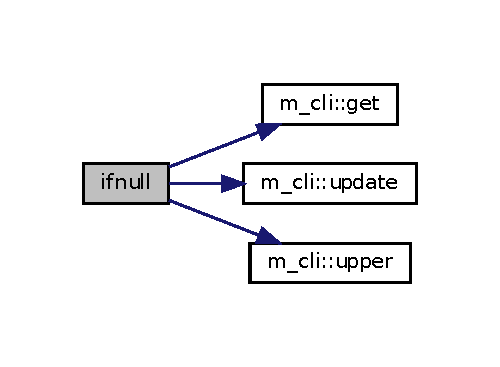
\includegraphics[width=240pt]{M__CLI_8f90_aa26f90016621d1ee43d3b5b66316532b_cgraph}
\end{center}
\end{figure}
Here is the caller graph for this function\+:\nopagebreak
\begin{figure}[H]
\begin{center}
\leavevmode
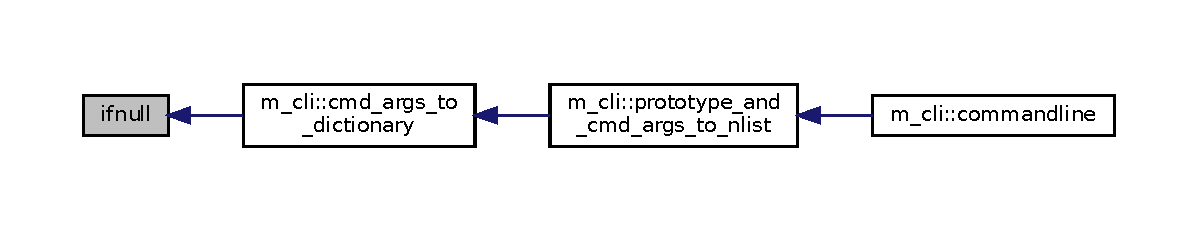
\includegraphics[width=350pt]{M__CLI_8f90_aa26f90016621d1ee43d3b5b66316532b_icgraph}
\end{center}
\end{figure}

\hypertarget{mainpage_8txt}{}\section{/home/urbanjs/venus/\+V600/github/\+M\+\_\+\+C\+L\+I/src/mainpage.txt File Reference}
\label{mainpage_8txt}\index{/home/urbanjs/venus/\+V600/github/\+M\+\_\+\+C\+L\+I/src/mainpage.\+txt@{/home/urbanjs/venus/\+V600/github/\+M\+\_\+\+C\+L\+I/src/mainpage.\+txt}}

%--- End generated contents ---

% Index
\backmatter
\newpage
\phantomsection
\clearemptydoublepage
\addcontentsline{toc}{chapter}{Index}
\printindex

\end{document}
